\documentclass[article,shortnames]{jss}

%% -- LaTeX packages and custom commands ------------------------------------
\usepackage{amsmath,amssymb}
\usepackage{booktabs}
\usepackage{longtable}
\usepackage{graphicx}

\newcommand{\pAm}{\{p_{Am}\}}
\newcommand{\pM}{[p_M]}
\newcommand{\EG}{[E_G]}

%% -- Article metadata ------------------------------------------------------
\author{Branimir K.~Hackenberger\\University of Osijek, SCIOM \And
        Tamara Djerdj\\University of Osijek \And
        Domagoj K.~Hackenberger\\Ru{\dj}er Bo{\v s}kovi{\'c} Institute}
\Plainauthor{Branimir K. Hackenberger, Tamara Djerdj,
             Domagoj K. Hackenberger}

\title{\pkg{BayesianDEB}: A Bayesian Framework for Dynamic Energy
       Budget Modelling in \proglang{R}}
\Plaintitle{BayesianDEB: A Bayesian Framework for Dynamic Energy Budget Modelling in R}
\Shorttitle{\pkg{BayesianDEB}: Bayesian DEB Framework in \proglang{R}}

\Abstract{
Dynamic Energy Budget (DEB) theory provides a mechanistic,
thermodynamically consistent description of how organisms acquire and
utilise energy throughout their life cycle.  The \proglang{R}~package
\pkg{BayesianDEB} embeds the standard DEB model within a Bayesian
state-space framework using \proglang{Stan} for Hamiltonian Monte
Carlo inference.  Four pre-written \proglang{Stan} programs cover
individual growth, growth with reproduction, hierarchical
multi-individual analysis, and toxicokinetic-toxicodynamic (TKTD)
models for ecotoxicology.  A declarative \proglang{R} interface
handles the full workflow without requiring \proglang{Stan}
programming.  We validate the individual growth model via
simulation-based calibration (500~replications) and show that DEB
rate parameters are largely prior-driven under single-individual
data, underscoring the importance of species-specific priors or
hierarchical pooling.  Real-data case studies demonstrate growth
estimation and DEBtox EC$_{50}$/NEC inference.
The package is available from
\url{https://sciom.r-universe.dev/BayesianDEB} and
\url{https://github.com/sciom/BayesianDEB}.
}

\Keywords{dynamic energy budget, Bayesian inference, \proglang{Stan},
  ecotoxicology, DEBtox, TKTD, hierarchical models, \proglang{R}}
\Plainkeywords{dynamic energy budget, Bayesian inference, Stan,
  ecotoxicology, DEBtox, TKTD, hierarchical models, R}

\Address{
  Branimir K.~Hackenberger\\
  Department of Biology\\
  Josip Juraj Strossmayer University of Osijek\\
  Osijek, Croatia\\
  and\\
  SCIOM d.o.o., Osijek, Croatia\\
  E-mail: \email{branimir@sciom.hr}\\
  URL: \url{https://github.com/sciom/BayesianDEB}\\[0.5em]
  %
  Tamara Djerdj\\
  Department of Biology\\
  Josip Juraj Strossmayer University of Osijek\\
  Osijek, Croatia\\[0.5em]
  %
  Domagoj K.~Hackenberger\\
  Ru{\dj}er Bo{\v s}kovi{\'c} Institute\\
  Zagreb, Croatia
}

%% -- Publication metadata (filled by JSS editors) --------------------------
\Volume{0}
\Issue{0}
\Month{}
\Year{}
\Submitdate{2026-04-06}
\Acceptdate{}

\begin{document}


%% ======================================================================
\section{Introduction} \label{sec:intro}
%% ======================================================================

Dynamic Energy Budget (DEB) theory \citep{Kooijman2010,
NisbetDEB2000, SousaDEB2008} provides a
mechanistic, thermodynamically grounded framework for describing
energy acquisition, storage, and allocation across the life cycle
of an organism, and is among the most widely applied metabolic
theories in ecology and ecotoxicology.  Its core state variables
--- reserve energy~$E$, structural volume~$V$, maturity~$E_H$, and
reproduction buffer~$E_R$ --- evolve according to an ordinary
differential equation (ODE) system governed by the $\kappa$-rule:
a fraction~$\kappa$ of mobilised reserve is allocated to somatic
maintenance and growth, while the remainder funds maturity maintenance
and reproduction.

Despite its theoretical elegance, DEB calibration has traditionally
relied on deterministic least-squares or maximum-likelihood
optimisation, as implemented in \pkg{DEBtool\_M}
\citep{MarquesAmP2018} and the Add-my-Pet (AmP) online estimation
tool.  This approach yields point estimates without formal uncertainty
quantification, cannot incorporate prior biological knowledge in a
principled way, and does not naturally extend to hierarchical data
structures where multiple individuals share species-level parameters
but differ in, for example, assimilation rate.

The combination of Bayesian inference with ODE-based models is, of
course, not new \citep{GelmanBDA2013}; \citet{BilloirBayesDEB2008}
pioneered Bayesian DEBtox calibration using Markov chain Monte Carlo (MCMC),
\citet{JohnsonDEB2015} applied custom samplers to DEB-based
thermal-response models, and \pkg{deBInfer}
\citep{deBInfer2017} provides a general Bayesian ODE framework in
\proglang{R}.  The contribution of the present work is not a new
statistical method but a \emph{domain-specific software
system} that makes three concrete advances over existing tools:
\begin{enumerate}
  \item \emph{Unified Bayesian workflow for DEB.}  No existing tool
    combines DEB ODE models, Hamiltonian Monte Carlo (HMC) inference, observation model
    switching, Arrhenius temperature correction, convergence
    diagnostics, posterior predictive checks, derived quantity
    estimation, and leave-one-out (LOO) cross-validation in a single
    \proglang{R} interface that requires no recompilation when
    switching observation families or prior specifications.  Users of
    \pkg{DEBtool\_M} or custom \proglang{Stan} code must assemble
    this workflow manually; \pkg{BayesianDEB} provides it
    out of the box for the four most common DEB applications.
  \item \emph{Reproducible, species-specific prior system grounded
    in the AmP collection.}  The function \code{prior\_species()}
    returns priors calibrated to AmP parameter estimates
    \citep{MarquesAmP2018} for common test species, bridging the
    gap between the world's largest DEB parameter database and
    Bayesian inference.  The prior-to-posterior contraction
    diagnostic (Section~\ref{sec:identifiability}) quantifies
    how much the data inform each parameter beyond the prior ---
    a transparency that deterministic calibration cannot offer.
  \item \emph{Inference validation for the individual growth model.}
    Simulation-based calibration (SBC;
    Section~\ref{sec:sbc}) with 500~replications and formal
    $\chi^2$ uniformity tests demonstrates, conditional on MCMC
    convergence, that the individual growth model is well-calibrated.
    SBC scripts for the hierarchical, growth-reproduction, and
    DEBtox models are also provided.  This level of algorithmic
    validation is uncommon in DEB calibration tools.
\end{enumerate}
Together, these advances lower the barrier to rigorous Bayesian DEB
modelling from expert \proglang{Stan} programming to a declarative
\proglang{R} call, while making identifiability limitations and
prior sensitivity explicit rather than hidden.

As we show in Section~\ref{sec:identifiability}, growth-only data
from a single individual cannot fully resolve the individual DEB
rate parameters; informative priors or hierarchical data
structures are needed for reliable inference.

The \pkg{BayesianDEB} package wraps four \proglang{Stan}
\citep{CarpenterStan2017} programs with a declarative \proglang{R}
interface, covering the four model types described in
Section~\ref{sec:theory}.  All models support switchable
observation families, Arrhenius temperature correction,
threading via \code{reduce\_sum}, and diagnostic tools
(Section~\ref{sec:design}).

This paper describes \pkg{BayesianDEB} version~0.1.3.  The package is
available from the SCIOM r-universe at
\url{https://sciom.r-universe.dev/BayesianDEB} and from GitHub
at \url{https://github.com/sciom/BayesianDEB}.


%% ======================================================================
\section{DEB theory and model formulation} \label{sec:theory}
%% ======================================================================

We summarise the DEB equations implemented in \pkg{BayesianDEB} and
discuss modelling choices; for a full treatment see
\citet{Kooijman2010}.  The standard DEB model is one of several
metabolic frameworks; alternatives include the ``standard'' and
``abj'' typified models in the AmP collection \citep{MarquesAmP2018},
net-production models, and various simplified formulations
\citep{JagerZimmer2012}.  \pkg{BayesianDEB} implements the standard
($\kappa$-rule) formulation, which is the most widely used and has the
largest empirical parameter base via AmP.

\subsection{Standard DEB: growth} \label{sec:growth}

\paragraph{Notation.}
DEB theory uses a specific bracket convention for parameters:
curly braces $\pAm$ denote surface-area-specific quantities,
square brackets $\pM$, $\EG$ denote volume-specific quantities,
and unbracketed symbols ($v$, $\kappa$) are dimensionless or have
other dimensions.  We follow this convention throughout.

Table~\ref{tab:notation} summarises the symbols, units, and roles of
all quantities used in this paper.

\begin{table}[t!]
\centering
\caption{Estimated parameters by model type (I = individual,
  G = growth\_repro, H = hierarchical, D = debtox).
  State variables ($E$, $V$, $E_R$, $D_w$) and fixed constants
  ($f$, $T$, $T_{\mathrm{ref}}$, $T_A$) are described in the text.}
\label{tab:notation}
\small
\begin{tabular}{lllc}
\toprule
Symbol & Description & Units & Models \\
\midrule
$\pAm$   & Max.\ assimilation rate   & J\,d$^{-1}$\,cm$^{-2}$ & all \\
$\pM$    & Somatic maintenance rate  & J\,d$^{-1}$\,cm$^{-3}$ & all \\
$\kappa$ & Allocation fraction       & --              & all \\
$v$      & Energy conductance        & cm\,d$^{-1}$   & all \\
$\EG$    & Cost of structure         & J\,cm$^{-3}$   & all \\
$E_0$, $L_0$ & Initial conditions   & J\,cm$^{-3}$, cm & all \\
$\sigma_L$ & Observation error SD   & cm              & all \\
$k_J$, $E_H^p$ & Maturity maint., puberty & d$^{-1}$, J & G \\
$k_R$, $\phi_R$ & Repro.\ conversion, overdisp. & --- & G,D \\
$k_d$    & Damage recovery rate      & d$^{-1}$       & D \\
$z_w$    & No-effect conc.\ (NEC)    & mg\,kg$^{-1}$  & D \\
$b_w$    & Effect intensity       & (mg\,kg$^{-1}$)$^{-1}$ & D \\
\bottomrule
\end{tabular}
\end{table}

The two core state variables are reserve energy $E$~(J) and structural
volume $V$~(cm$^3$), with structural length $L = V^{1/3}$.  Under
constant food availability characterised by the scaled functional
response $f \in [0, 1]$, the energy fluxes are:
\begin{align}
  \dot{p}_A &= f \, \pAm \, L^2,  \label{eq:pA} \\
  \dot{p}_C &= \frac{E \, v \, L}{E + \EG \, V},  \label{eq:pC} \\
  \dot{p}_M &= \pM \, V,  \label{eq:pM}
\end{align}
where $\pAm$ is the surface-area-specific maximum assimilation rate
(J\,d$^{-1}$\,cm$^{-2}$), $v$ is the energy conductance
(cm\,d$^{-1}$), $\EG$ is the specific cost of structure
(J\,cm$^{-3}$), and $\pM$ is the volume-specific somatic maintenance
rate (J\,d$^{-1}$\,cm$^{-3}$).  Note that the mobilisation flux
$\dot{p}_C$ (Equation~\ref{eq:pC}) is the total catabolic power
drawn from reserve; it is subsequently partitioned by the
$\kappa$-rule in the state equations below.  The state equations
are:
\begin{align}
  \frac{dE}{dt} &= \dot{p}_A - \dot{p}_C,  \label{eq:dE} \\
  \frac{dV}{dt} &= \frac{\kappa \, \dot{p}_C - \dot{p}_M}{\EG},
    \label{eq:dV}
\end{align}
where $\kappa$ is the allocation fraction to soma.  At steady state
($dV/dt = 0$, $dE/dt = 0$), the ultimate structural length is
$L_\infty = f \, \kappa \, \pAm / \pM$.

\paragraph{Edge cases.}
When $\kappa \dot{p}_C < \dot{p}_M$ (starvation), growth ceases and
the organism draws on structure for maintenance; in our implementation
$dV/dt$ is clamped to zero to prevent negative structural volume.
When $\kappa \to 0$, nearly all mobilised energy goes to reproduction
and growth is negligible; when $\kappa \to 1$, reproduction ceases.
The Beta prior on $\kappa$ (default $\mathrm{Beta}(2,2)$) regularises
the posterior away from these boundary cases.

\paragraph{Initial conditions.}
Both $E_0$ (initial reserve density, J\,cm$^{-3}$) and $L_0$
(initial structural length) are estimated with log-normal priors.
The total initial reserve is $E(0) = E_0 L_0^3$.  Estimating $E_0$
freely avoids assuming energy steady state, which may not hold for
hatchlings.  In the hierarchical model, $E_0$ is shared across
individuals while $L_{0,j}$ varies.

\paragraph{ODE stiffness and solver choice.}
DEB systems are mildly stiff due to the time-scale separation between
fast reserve dynamics and slow structural growth.  The mobilisation
flux $\dot{p}_C = EvL / (E + \EG V)$ creates stiffness when $E \gg
\EG V$ (near steady-state reserve).  We use the BDF (backward
differentiation formula) solver \code{ode\_bdf\_tol} with tolerances
$10^{-6}$, which is standard for mildly stiff biological ODE systems.
The explicit Runge-Kutta solver (\code{ode\_rk45}) was also tested:
it produced identical trajectories for well-conditioned parameter
regions but required approximately $2\times$ more function evaluations
and occasionally failed for extreme parameter combinations during MCMC
warmup.  The BDF solver was therefore chosen as the safer default.

\subsection{Growth with reproduction} \label{sec:repro}

For post-pubertal organisms ($E_H \geq E_H^p$), adding the
reproduction buffer $E_R$~(J) yields a 3-state model:
\begin{equation}
  \frac{dE_R}{dt} = (1 - \kappa) \, \dot{p}_C - k_J \, E_H^p,
    \label{eq:dR}
\end{equation}
where $k_J$ is the maturity maintenance rate coefficient and $E_H^p$
is maturity at puberty (treated as a known constant, not a state
variable, since the model describes post-pubertal growth only).  Offspring counts over an interval
$[t_s, t_e]$ are modelled as
$R \sim \mathrm{NegBin}_2(\mu = k_R \, \Delta E_R,\, \phi)$,
where $\Delta E_R = E_R(t_e) - E_R(t_s)$, $k_R$ is the buffer-to-offspring
conversion rate (offspring\,J$^{-1}$), $\mu$ is the expected count, and
$\phi > 0$ is the overdispersion parameter.  This uses \proglang{Stan}'s
\code{neg\_binomial\_2} parametrisation, where $\mathrm{E}[R] = \mu$
and $\mathrm{Var}[R] = \mu + \mu^2/\phi$; as
$\phi \to \infty$ the distribution converges to
$\mathrm{Poisson}(\mu)$.

\subsection{DEBtox: toxicokinetic-toxicodynamic extension}
\label{sec:debtox}

The DEBtox framework \citep{JagerDEBtox2006, JagerZimmer2012}, part
of the broader toxicokinetic-toxicodynamic (TKTD) family that includes
the General Unified Threshold model of Survival (GUTS) for survival
\citep{JagerGUTS2011}, adds a scaled internal damage variable~$D_w$:
\begin{equation}
  \frac{dD_w}{dt} = k_d \bigl(\max(C_w - z_w, 0) - D_w\bigr),
    \label{eq:Dw}
\end{equation}
where $k_d$ is the damage recovery rate, $C_w$ is the external
concentration, and $z_w$ is the no-effect concentration (NEC).  The
damage causes a stress factor $s = b_w \, D_w$ that reduces
assimilation: $\dot{p}_A \leftarrow \dot{p}_A \cdot \max(1 - s, 0)$.
The reproduction buffer in the DEBtox model follows a simplified form
$dE_R/dt = (1 - \kappa)\dot{p}_C$ (omitting the maturity maintenance
term $k_J E_H^p$ from Equation~\ref{eq:dR}), since the stress on
assimilation already captures the dominant toxicant effect on
reproduction; consequently, $k_J$ and $E_H^p$ are not parameters of
the DEBtox model.
At steady state, $D_w = C_w - z_w$ for $C_w > z_w$, so the
EC$_{50}$ for 50\% assimilation reduction is:
\begin{equation}
  \mathrm{EC}_{50} = z_w + \frac{0.5}{b_w}.
    \label{eq:EC50}
\end{equation}

\subsection{Arrhenius temperature correction} \label{sec:arrhenius}

All rate parameters scale with temperature by the factor
$c_T = \exp(T_A / T_{\mathrm{ref}} - T_A / T)$
\citep[Eq.~1.2]{Kooijman2010}, where $T_A$ is the Arrhenius
temperature (species-specific, typically 6000--12\,000~K).  In
\pkg{BayesianDEB}, the correction is applied inside the
\proglang{Stan} ODE to $\pAm$, $\pM$, $v$, $k_J$, and $k_d$;
the estimated parameters correspond to the reference temperature
$T_{\mathrm{ref}}$.

\subsection{Hierarchical structure} \label{sec:hierarchical}

When data from multiple individuals are available, a lognormal random
effect on $\pAm$ is introduced:
\begin{equation}
  \log \pAm_j = \mu_{\log \pAm} + \sigma_{\log \pAm} \cdot z_j,
  \qquad z_j \sim \mathcal{N}(0, 1),
    \label{eq:hier}
\end{equation}
using a non-centred parameterisation to avoid pathological funnel
geometry \citep{BetancourtHierarchical2015}.
The shared parameters $\pM$, $\kappa$, $v$, $\EG$ are estimated from
all individuals jointly (partial pooling).

\paragraph{Why random effects on $\pAm$ only?}
In DEB theory, $\pAm$ is the parameter most strongly linked to
individual phenotypic variation: it determines food uptake capacity and
scales with structural surface area, which varies among individuals
due to differences in condition, microhabitat, and genotype.  The
energy conductance~$v$, maintenance~$\pM$, and costs~$\EG$ are
typically more conserved within a species \citep{Kooijman2010,
MarquesAmP2018}.  We acknowledge that individual variation in
$\kappa$ and $L_0$ is also documented empirically; however,
placing random effects on all parameters simultaneously would
create a high-dimensional, poorly identified model for typical DEB
dataset sizes (5--30~individuals with 5--15~time points each).
Our contraction analysis (Section~\ref{sec:identifiability}) shows
that even shared parameters are weakly identified from growth-only
data; adding per-individual variation on multiple parameters would
exacerbate this.  The single-random-effect design is therefore a
deliberate parsimony choice that provides partial pooling on the
most variable parameter while keeping the model identifiable.
Extension to multivariate random effects on $(\pAm, \kappa)$ or
$(\pAm, L_0)$, potentially with informative LKJ priors on the
correlation matrix, is planned for a future version.


%% ======================================================================
\section{Bayesian state-space formulation} \label{sec:statespace}
%% ======================================================================

We now formalise the statistical model.  Let
$\mathbf{x}(t) = (E(t), V(t))^\top$ denote the latent DEB state
(extended to $(E, V, E_R)^\top$ or $(E, V, E_R, D_w)^\top$
for the reproduction and DEBtox models), and let
$\boldsymbol{\theta}$ collect the DEB parameters.

\subsection{Process model}

The latent state evolves deterministically according to the ODE:
\begin{equation}
  \frac{d\mathbf{x}}{dt} = \mathbf{f}(\mathbf{x}, \boldsymbol{\theta},
  f, C_w), \qquad \mathbf{x}(0) = \mathbf{x}_0(\boldsymbol{\theta}),
  \label{eq:ode_general}
\end{equation}
where $\mathbf{f}$ is defined by
Equations~\eqref{eq:dE}--\eqref{eq:dV} (growth),
\eqref{eq:dR} (reproduction), or \eqref{eq:Dw} (DEBtox), and
$\mathbf{x}_0$ depends on initial conditions $(E_0, L_0)$.

\subsection{Observation model}

Given the ODE solution $\hat{L}_i = [\mathbf{x}(t_i)]_V^{1/3}$,
the growth observations are conditionally independent:
\begin{equation}
  L_i^{\mathrm{obs}} \mid \hat{L}_i, \sigma_L \;\sim\;
  \begin{cases}
    \mathcal{N}(\hat{L}_i,\, \sigma_L) & \text{(Gaussian)}, \\
    \mathrm{LogNormal}(\log\hat{L}_i,\, \sigma_L) & \text{(log-normal)}, \\
    t_\nu(\hat{L}_i,\, \sigma_L) & \text{(Student-}t\text{)}.
  \end{cases}
  \label{eq:obs_L}
\end{equation}
For reproduction, interval offspring counts use \proglang{Stan}'s
mean-overdispersion parametrisation
(\code{neg\_binomial\_2}):
\begin{equation}
  R_k \mid \mu_k, \phi \;\sim\;
  \mathrm{NegBin}_2(\mu_k,\, \phi)
  \quad\text{or}\quad
  \mathrm{Poisson}(\mu_k),
  \qquad \mu_k = k_R \, \Delta E_{R,k},
  \label{eq:obs_R}
\end{equation}
where $\mathrm{E}[R_k] = \mu_k$ and $\mathrm{Var}[R_k] = \mu_k +
\mu_k^2 / \phi$.

\subsection{Prior model}

The full prior factorises as:
\begin{equation}
  p(\boldsymbol{\theta}) = p(\pAm) \, p(\pM) \, p(\kappa) \, p(v) \,
  p(\EG) \, p(E_0) \, p(L_0) \, p(\sigma_L) \, [\text{model-specific}].
  \label{eq:prior}
\end{equation}
Default prior families are: $\pAm, \pM, v, \EG \sim
\mathrm{LogNormal}$; $\kappa \sim \mathrm{Beta}$; $\sigma_L \sim
\mathrm{HalfNormal}$ \citep[following the recommendations
of][]{GelmanPriorVariance2006}.  Hyperparameters are calibrated
against the AmP collection ranges \citep{MarquesAmP2018} and passed
to \proglang{Stan} as data, so that changing priors does not require
recompilation.

\paragraph{Prior calibration rationale.}
Table~\ref{tab:priors} shows the generic default hyperparameters
and their implied 95\% prior mass ranges.  These defaults
(from \code{prior\_default()}) are deliberately wide
($\sigma = 1.0$) to accommodate any species; they are
\emph{not} suitable for quantitative inference without
tightening (see Section~\ref{sec:identifiability}).

For common test species, the function \code{prior\_species()} returns
priors calibrated to the AmP collection \citep{MarquesAmP2018},
with $\sigma = 0.3$ for well-characterised parameters:
\begin{CodeChunk}
\begin{CodeInput}
R> prior_species("Eisenia_fetida")
\end{CodeInput}
\begin{CodeOutput}
  p_Am:    LogNormal(1.61, 0.3)
  p_M:     LogNormal(-0.69, 0.3)
  kappa:   Beta(5, 2)
  v:       LogNormal(-3.91, 0.5)
  E_G:     LogNormal(8.39, 0.3)
  sigma_L: HalfNormal(0.05)
\end{CodeOutput}
\begin{CodeInput}
R> prior_species("Daphnia_magna", type = "debtox")
\end{CodeInput}
\end{CodeChunk}
\noindent
Built-in species include \emph{Eisenia fetida}, \emph{E.~andrei},
\emph{Folsomia candida}, \emph{Daphnia magna}, and
\emph{Lumbricus rubellus}.  Users working with other species should
construct custom priors from the relevant AmP entry.  We recommend
always conducting a prior sensitivity analysis
(Section~\ref{sec:identifiability}).

\begin{table}[t!]
\centering
\caption{Default prior specifications and implied ranges, compared
  with AmP empirical ranges for earthworms and springtails.}
\label{tab:priors}
\begin{tabular}{llrrl}
\toprule
Parameter & Prior family & $\mu$ / $a$ & $\sigma$ / $b$ &
  95\% prior range \\
\midrule
$\pAm$    & LogNormal & 1.0  & 1.0  & 0.4--20 \\
$\pM$     & LogNormal & $-$1.0 & 1.0 & 0.04--2 \\
$\kappa$  & Beta      & 2    & 2    & 0.09--0.91 \\
$v$       & LogNormal & $-$1.5 & 1.0 & 0.02--1 \\
$\EG$     & LogNormal & 6.0  & 1.0  & 100--3000 \\
$\sigma_L$ & HalfNormal & 0 & 0.1 & 0--0.2 \\
\bottomrule
\end{tabular}
\end{table}

\subsection{Joint posterior}

The posterior is:
\begin{equation}
  p(\boldsymbol{\theta} \mid \mathbf{y}) \;\propto\;
  p(\boldsymbol{\theta}) \prod_{i=1}^{N_L}
  p(L_i^{\mathrm{obs}} \mid \hat{L}_i(\boldsymbol{\theta}), \sigma_L)
  \prod_{k=1}^{N_R}
  p(R_k \mid \Delta E_{R,k}(\boldsymbol{\theta}), k_R, \phi),
  \label{eq:posterior}
\end{equation}
sampled via the No-U-Turn Sampler \citep[NUTS;][]{HoffmanNUTS2014}
with a stiff BDF ODE solver evaluated at each leapfrog step.

\subsection{Hierarchical extension}

For $J$ individuals with individual random effects on $\pAm$, the
hierarchical model adds population-level hyperparameters
$\mu_{\log \pAm}$ and $\sigma_{\log \pAm}$:
\begin{equation}
  \log \pAm_j \mid \mu, \sigma \;\sim\; \mathcal{N}(\mu, \sigma),
  \qquad j = 1, \ldots, J.
  \label{eq:hier_formal}
\end{equation}
The non-centred parameterisation (Equation~\ref{eq:hier}) is used
as described in Section~\ref{sec:hierarchical}.


%% ======================================================================
\section[BayesianDEB: software design]{%
  \pkg{BayesianDEB}: software design} \label{sec:design}
%% ======================================================================

\subsection{Architecture} \label{sec:architecture}

The package follows the domain-specific \proglang{Stan} wrapper
pattern established by \pkg{brms} \citep{Burknerbrms2017}, with
\pkg{cmdstanr} \citep{Gabrycmdstanr2024} as the compilation and
sampling back-end.  It consists of three layers:
\begin{description}
  \item[\proglang{Stan} models.] Four pre-written \code{.stan} programs
    in \code{inst/stan/}, implementing the DEB ODE system with
    the variadic \code{ode\_bdf\_tol} solver (BDF, tolerances
    $10^{-6}$).  The hierarchical and DEBtox models use
    \code{reduce\_sum} for within-chain parallelism
    (Section~\ref{sec:threading}).  Observation model
    switching is controlled by integer flags
    in the \proglang{Stan} data block, avoiding recompilation when
    changing observation families or prior hyperparameters.
  \item[\proglang{R} interface.] Exported functions for data
    preparation, model specification, MCMC fitting, diagnostics,
    posterior predictive checks, derived quantities,
    LOO cross-validation, prior predictive simulation,
    and reproducibility reporting (see Table~\ref{tab:comparison}
    and the package documentation for the full API).  All
    functions use S3 classes (\code{bdeb\_data},
    \code{bdeb\_model}, \code{bdeb\_fit}); all three support
    \code{print}, and \code{bdeb\_fit} additionally provides
    \code{plot}, \code{summary}, \code{coef}, and
    \code{predict} methods.
  \item[Prior system.] Six \code{prior\_*()} constructor functions
    (log-normal, beta, half-normal, half-Cauchy, exponential,
    normal) encode distribution choices as lightweight S3 objects.
    Weakly informative defaults calibrated against the AmP
    collection \citep{MarquesAmP2018} are provided via
    \code{prior\_default()}.
\end{description}

\paragraph{\proglang{Stan} code excerpt.}
The following annotated excerpt from
\code{bdeb\_individual\_growth.stan} shows the DEB ODE
implementation:
\begin{CodeChunk}
\begin{CodeInput}
functions {
  vector deb_growth_ode(real t, vector x,
      real p_Am, real p_M, real kappa, real v_, real E_G, real f) {
    real E = x[1]; real V = x[2];
    real L = pow(V, 1.0/3.0);
    real p_A = f * p_Am * L * L;
    real p_C = E * v_ * L / (E + E_G * V);
    real dE = p_A - p_C;
    real dV = (kappa * p_C - p_M * V) / E_G;
    return [dE, dV]';
  }
}
\end{CodeInput}
\end{CodeChunk}
\noindent
The \code{model} block applies priors whose hyperparameters are
passed as \proglang{Stan} data (avoiding recompilation) and
dispatches the observation likelihood via an integer flag
(\code{obs\_growth}: 1=normal, 2=lognormal, 3=Student-$t$).  The
full programs (137--219~lines each) include ODE solving via
\code{ode\_bdf\_tol} and generated quantities for posterior
predictive checking (PPC) and LOO-CV.

\subsection{Workflow} \label{sec:workflow}

The recommended workflow follows the iterative Bayesian modelling cycle
of \citet[Ch.~6]{GelmanBDA2013}:
\begin{enumerate}
  \item Prepare and validate data with \code{bdeb\_data()}.
  \item Specify model, priors, and observation family with
    \code{bdeb\_model()}.
  \item Fit via MCMC with \code{bdeb\_fit()}.
  \item Check convergence with \code{bdeb\_diagnose()}
    ($\hat{R}$, effective sample size (ESS), divergences;
    \citealp{VehtariRhat2021}).
    Inspect parameter estimates with \code{bdeb\_summary()} (or
    the S3 \code{summary()} method).
  \item Perform posterior predictive checks with \code{bdeb\_ppc()}
    \citep{GabryPPC2019}.
  \item Compute derived quantities with \code{bdeb\_derived()}.
  \item Generate predictions at new conditions with
    \code{bdeb\_predict()} (or the S3 \code{predict()} method).
  \item Compare models via \code{bdeb\_loo()}
    \citep{VehtariLOO2017}.
  \item Iterate: revise priors or model structure as needed.
\end{enumerate}
\noindent
Steps~5 and~7 (PPC and LOO) require \code{L\_rep} and
\code{log\_lik} arrays from \proglang{Stan}'s \code{generated
quantities} block and are therefore available only for the
\code{"individual"} and \code{"growth\_repro"} models.  The
\code{"hierarchical"} and \code{"debtox"} models use
\code{reduce\_sum}, which precludes per-observation generated
quantities; for these models, trajectory plots from \proglang{R}-side forward
simulation (\code{plot(fit, type = "trajectory")}) serve as the
primary model-checking tool.

\paragraph{Data format.}
The \code{growth} data frame must contain columns \code{id},
\code{time} (days), and \code{length} (structural cm).  For
\code{"growth\_repro"}, an additional \code{reproduction} data frame
with \code{id}, \code{t\_start}, \code{t\_end}, and \code{count} is
required.  The \code{"debtox"} model needs a \code{concentration}
column.  Input validation checks types, ranges, and consistency.

\paragraph{API summary.}
Table~\ref{tab:api} lists the main exported functions (32~functions
and 12~S3 methods in total).

\begin{table}[t!]
\centering
\caption{Main exported functions, grouped by workflow phase.}
\label{tab:api}
\small
\begin{tabular}{lll}
\toprule
Phase & Function(s) & Purpose \\
\midrule
Data      & \code{bdeb\_data} & Prepare \& validate data \\
Model     & \code{bdeb\_model}, \code{bdeb\_tox}, \code{bdeb\_fit}
                                                & Specify, wrap, fit \\
Priors    & \code{prior\_lognormal}, \ldots\ (6) & Distribution constructors \\
          & \code{prior\_default}, \code{prior\_species}
                                                & Defaults \& AmP priors \\
Obs.      & \code{obs\_normal}, \ldots\ (5)     & Likelihood constructors \\
Diagnostics & \code{bdeb\_diagnose}, \code{bdeb\_summary}, \code{bdeb\_loo}
                                                & Convergence \& comparison \\
Posterior & \code{bdeb\_derived}, \code{bdeb\_ppc}, \code{bdeb\_predict}
                                                & Derived quantities, PPC \\
          & \code{bdeb\_ec50}, \code{bdeb\_prior\_predictive}
                                                & EC$_{50}$/NEC, prior pred. \\
Plots     & \code{plot(fit, ...)}, \code{plot\_dose\_response}
                                                & 5~plot types + dose-resp. \\
Utilities & \code{deb\_simulate}, \code{debtox\_simulate}
                                                & Standalone ODE simulators \\
          & \code{arrhenius}, \code{deb\_fluxes}
                                                & Temperature, energy fluxes \\
\bottomrule
\end{tabular}
\end{table}

\subsection{Observation models} \label{sec:obs}

The observation model is selected via constructor functions passed to
the \code{observation} argument of \code{bdeb\_model()}:
\begin{CodeChunk}
\begin{CodeInput}
R> mod <- bdeb_model(dat, type = "individual",
+    observation = list(growth = obs_student_t(nu = 5)))
\end{CodeInput}
\end{CodeChunk}
The choice is encoded as an integer flag in the \proglang{Stan} data
block (\code{obs\_growth = 1/2/3}, \code{obs\_repro = 1/2}) and
dispatched via conditional blocks in the model and generated quantities
sections.  This avoids recompilation when switching families.

\subsection{Temperature correction} \label{sec:temp_impl}

If a \code{temperature} list is supplied to \code{bdeb\_model()}, the
Arrhenius correction factor $c_T$ is computed in the \proglang{Stan}
\code{transformed data} block and applied to all rate parameters inside
the ODE.  The posterior gives estimates at $T_{\mathrm{ref}}$, making
results comparable across experiments at different temperatures.

\subsection{Within-chain parallelism} \label{sec:threading}

The hierarchical and DEBtox models distribute per-individual (or
per-group) ODE solves across threads via \proglang{Stan}'s
\code{reduce\_sum}.  The \code{threads\_per\_chain} argument in
\code{bdeb\_fit()} controls this:
\begin{CodeChunk}
\begin{CodeInput}
R> fit <- bdeb_fit(mod, chains = 4, threads_per_chain = 4)
\end{CodeInput}
\end{CodeChunk}

\subsection{Testing} \label{sec:testing}

The package includes 18~\pkg{testthat} test files covering unit,
integration, API contract, and scientific consistency checks.
MCMC-dependent tests use mock objects.  The SBC scripts
(Section~\ref{sec:sbc}) provide additional validation.


%% ======================================================================
\section{Illustrations} \label{sec:illustrations}
%% ======================================================================

We illustrate all four model types: individual growth, growth with
reproduction, hierarchical multi-individual growth, and DEBtox.

\subsection[Individual growth: Eisenia fetida]{%
  Individual growth: \emph{Eisenia fetida}} \label{sec:ex_ind}

The bundled \code{eisenia\_growth} dataset contains simulated weekly
length measurements for 21~individuals of the earthworm \emph{Eisenia
fetida} over 84~days, using AmP parameters ($\pAm = 5.0$,
$\pM = 0.5$, $\kappa = 0.75$, $v = 0.2$, $\EG = 400$) with
individual variation in $\pAm$ (CV~$\approx$~10\%) and Gaussian
measurement error ($\sigma_L = 0.015$~cm).

\begin{CodeChunk}
\begin{CodeInput}
R> library("BayesianDEB")
R> data("eisenia_growth")
R> df1 <- eisenia_growth[eisenia_growth$id == 5, ]
R> dat <- bdeb_data(growth = df1, f_food = 1.0)
R> dat
\end{CodeInput}
\begin{CodeOutput}
-- BDEB Data --
i Individuals: 1
i Endpoints: growth
i Functional response (f): 1
> Growth: 13 observations, t = [0, 84]
\end{CodeOutput}
\begin{CodeInput}
R> mod <- bdeb_model(dat, type = "individual",
+    priors = list(
+      p_Am    = prior_lognormal(mu = 1.5, sigma = 0.5),
+      kappa   = prior_beta(a = 3, b = 2),
+      sigma_L = prior_halfnormal(sigma = 0.05)))
R> mod
\end{CodeInput}
\begin{CodeOutput}
-- BDEB Model Specification --
i Type: individual
i Stan model: bdeb_individual_growth
i Individuals: 1
i Endpoints: growth
-- Priors
>   p_Am: LogNormal(1.5, 0.5)
>   kappa: Beta(3.0, 2.0)
>   sigma_L: HalfNormal(0.05)
>   p_M: LogNormal(-1.0, 1.0)    [default]
>   v: LogNormal(-1.5, 1.0)      [default]
>   E_G: LogNormal(6.0, 1.0)     [default]
>   E0: LogNormal(0.0, 1.0)      [default]
>   L0: LogNormal(-2.0, 1.0)     [default]
\end{CodeOutput}
\begin{CodeInput}
R> pp <- bdeb_prior_predictive(mod, n_draws = 500, seed = 1)
R> plot(pp)
\end{CodeInput}
\end{CodeChunk}
\noindent
The prior predictive check simulates DEB trajectories from the prior
alone (no data); the resulting fan should envelope the observations
without spanning orders of magnitude.

\begin{CodeChunk}
\begin{CodeInput}
R> fit <- bdeb_fit(mod, chains = 4, iter_sampling = 2000,
+    adapt_delta = 0.9, seed = 42)
R> bdeb_diagnose(fit)
\end{CodeInput}
\begin{CodeOutput}
  variable  mean    sd median    5%    95% rhat ess_bulk ess_tail
      p_Am  5.06  2.65   4.47  1.96 10.00 1.00     8268     5682
       p_M  0.56  0.65   0.36  0.07  1.74 1.00     7795     5381
     kappa  0.59  0.20   0.60  0.25  0.89 1.00     6657     4667
         v  0.30  0.35   0.20  0.05  0.89 1.00     4826     5278
       E_G   574   471    454   130  1410  1.00     3717     4363
   sigma_L 0.013 0.003  0.013 0.009 0.019 1.00     5525     4428
\end{CodeOutput}
\begin{CodeInput}
R> plot(fit, type = "trajectory", n_draws = 200, seed = 1)
\end{CodeInput}
\end{CodeChunk}
\noindent
All $\hat{R} \leq 1.01$ and bulk ESS~$>$~3000.  The initial
length $L_0 = 0.116$~cm matches the first observation; rate
parameters have wider posteriors reflecting the identifiability
constraints of Section~\ref{sec:identifiability}.

The derived ultimate length and von Bertalanffy growth rate are
obtained with full posterior uncertainty propagation:
\begin{CodeChunk}
\begin{CodeInput}
R> bdeb_derived(fit, quantities = c("L_m", "L_inf", "k_M",
+    "g", "growth_rate"), f = 1.0)
\end{CodeInput}
\begin{CodeOutput}
# A draws_df: 8000 draws, 5 variables
     L_m L_inf     k_M      g growth_rate
1    4.5   4.5 0.00155  33.90    0.000503
2    8.7   8.7 0.00084  18.80    0.000270
3   10.0  10.0 0.00042  93.20    0.000140
...
\end{CodeOutput}
\end{CodeChunk}
All formulas follow \citet[Table~3.1]{Kooijman2010}: $L_m = \kappa
\pAm / \pM$, $L_\infty = f \cdot L_m$, $k_M = \pM / \EG$,
$g = \EG \, v / (\kappa \, \pAm)$, $\dot{r}_B = k_M \, g / (3(f + g))$.

\paragraph{Model comparison via LOO.}
The observation model can be compared via approximate
leave-one-out cross-validation \citep{VehtariLOO2017}:
\begin{CodeChunk}
\begin{CodeInput}
R> mod_ln <- bdeb_model(dat, type = "individual",
+    observation = list(growth = obs_lognormal()),
+    priors = list(
+      p_Am  = prior_lognormal(mu = 1.5, sigma = 0.5),
+      kappa = prior_beta(a = 3, b = 2),
+      sigma_L = prior_halfnormal(sigma = 0.05)))
R> fit_ln <- bdeb_fit(mod_ln, chains = 4,
+    iter_sampling = 2000, adapt_delta = 0.9, seed = 42)
R> loo_gauss <- bdeb_loo(fit)
R> loo_ln    <- bdeb_loo(fit_ln)
R> loo::loo_compare(list(gaussian = loo_gauss,
+    lognormal = loo_ln))
\end{CodeInput}
\begin{CodeOutput}
          elpd_diff se_diff
gaussian   0.0       0.0
lognormal -0.7       1.1
\end{CodeOutput}
\end{CodeChunk}
\noindent
The Gaussian model is marginally preferred (higher expected log
predictive density, ELPD), but the
difference ($\Delta$ELPD $= -0.7$, SE $= 1.1$) is well within one
standard error, indicating that neither observation model is
decisively better for this dataset.

\subsection[Growth with reproduction: Folsomia candida]{%
  Growth with reproduction: \emph{Folsomia candida}}
  \label{sec:ex_repro}

The \code{"growth\_repro"} model extends the individual growth model
with a reproduction buffer (Section~\ref{sec:repro}), fitting both
growth and offspring count data simultaneously.  We illustrate the
interface using simulated data for the springtail \emph{Folsomia
candida}: 28~days of bi-weekly structural length measurements
paired with a single offspring count over the full interval, mimicking
a standard ISO~11267 reproduction test.

\begin{CodeChunk}
\begin{CodeInput}
R> growth_fc <- data.frame(id = 1,
+    time = seq(0, 28, by = 2),
+    length = c(0.048, 0.053, 0.058, 0.063, 0.067, 0.071,
+               0.075, 0.078, 0.081, 0.084, 0.086, 0.088,
+               0.089, 0.090, 0.091))
R> repro_fc <- data.frame(id = 1, t_start = 0,
+    t_end = 28, count = 118)
R> dat_gr <- bdeb_data(growth = growth_fc,
+    reproduction = repro_fc, f_food = 1.0)
R> mod_gr <- bdeb_model(dat_gr, type = "growth_repro",
+    priors = prior_species("Folsomia_candida",
+      type = "growth_repro"),
+    observation = list(growth = obs_normal(),
+      reproduction = obs_negbinom()))
R> fit_gr <- bdeb_fit(mod_gr, chains = 4,
+    iter_sampling = 2000, adapt_delta = 0.9, seed = 42)
R> bdeb_diagnose(fit_gr)
\end{CodeInput}
\end{CodeChunk}

\noindent
The additional parameters $k_J$ (maturity maintenance rate), $E_H^p$
(maturity at puberty), $k_R$ (reproduction efficiency), and $\phi_R$
(negative binomial overdispersion) are estimated alongside the core
DEB parameters.  Note that a single offspring count (as in the
example above) provides limited information for the four
reproduction parameters; multiple counting intervals
(e.g., weekly counts over a 28-day test) substantially improve
identifiability of $k_R$ and $\phi_R$.  The observation model can
be switched to Poisson for reproduction via \code{obs\_poisson()}
without recompilation.
LOO cross-validation can separately evaluate the growth and
reproduction likelihood components:

\begin{CodeChunk}
\begin{CodeInput}
R> bdeb_loo(fit_gr, endpoint = "growth")
R> bdeb_loo(fit_gr, endpoint = "reproduction")
R> bdeb_loo(fit_gr, endpoint = "all")
\end{CodeInput}
\end{CodeChunk}

\subsection{Hierarchical model} \label{sec:ex_hier}

\begin{CodeChunk}
\begin{CodeInput}
R> dat_all <- bdeb_data(growth = eisenia_growth, f_food = 1.0)
R> mod_h <- bdeb_model(dat_all, type = "hierarchical",
+    priors = list(
+      mu_log_p_Am    = prior_normal(mu = 1.5, sigma = 0.5),
+      sigma_log_p_Am = prior_exponential(rate = 2)))
R> fit_h <- bdeb_fit(mod_h, chains = 4, adapt_delta = 0.95,
+    threads_per_chain = 4, seed = 123)
R> bdeb_diagnose(fit_h)
R> plot(fit_h, type = "trajectory", n_draws = 50, seed = 1)
\end{CodeInput}
\end{CodeChunk}

The trajectory plot produces a faceted display with one panel per
individual, showing posterior predicted curves overlaid on observed data.
The hierarchical model yields narrower credible intervals for shared
parameters than the individual fit because it pools information across
21~organisms.

\subsection{DEBtox analysis} \label{sec:ex_debtox}

\begin{CodeChunk}
\begin{CodeInput}
R> data("debtox_growth")
R> conc_map <- setNames(unique(debtox_growth$concentration),
+    as.character(unique(debtox_growth$concentration)))
R> dat_tox <- bdeb_data(growth = debtox_growth,
+    concentration = conc_map, f_food = 1.0)
R> mod_tox <- bdeb_tox(dat_tox, stress = "assimilation",
+    priors = list(
+      z_w = prior_lognormal(mu = 2.5, sigma = 1.0),
+      b_w = prior_lognormal(mu = -5.0, sigma = 2.0)))
R> fit_tox <- bdeb_fit(mod_tox, chains = 4, adapt_delta = 0.95,
+    threads_per_chain = 2, seed = 77)
R> bdeb_ec50(fit_tox, prob = 0.95)
R> plot_dose_response(fit_tox, n_draws = 100, seed = 1)
\end{CodeInput}
\end{CodeChunk}

The EC$_{50}$ is computed analytically in \proglang{Stan}'s
\code{generated quantities} block as $z_w + 0.5 / b_w$, giving the
full posterior distribution without post-hoc root-finding.

\paragraph{Real-data DEBtox: cadmium toxicity to \emph{E.~andrei}.}
To demonstrate the DEBtox model on experimental data, we analyse
the growth of \emph{Eisenia andrei} exposed to cadmium (0, 10, 32,
100, 320~mg\,Cd\,kg$^{-1}$ in natural soil) from
\citet{VanGestel1991}, obtained via the EGrowth database
\citep{MathieuEGrowth2018}.  The dataset comprises 5~concentration
groups with 7~time points each over 85~days (group-mean body mass
converted to structural length and bundled as \code{eisenia\_cd}).

\begin{figure}[t!]
\centering
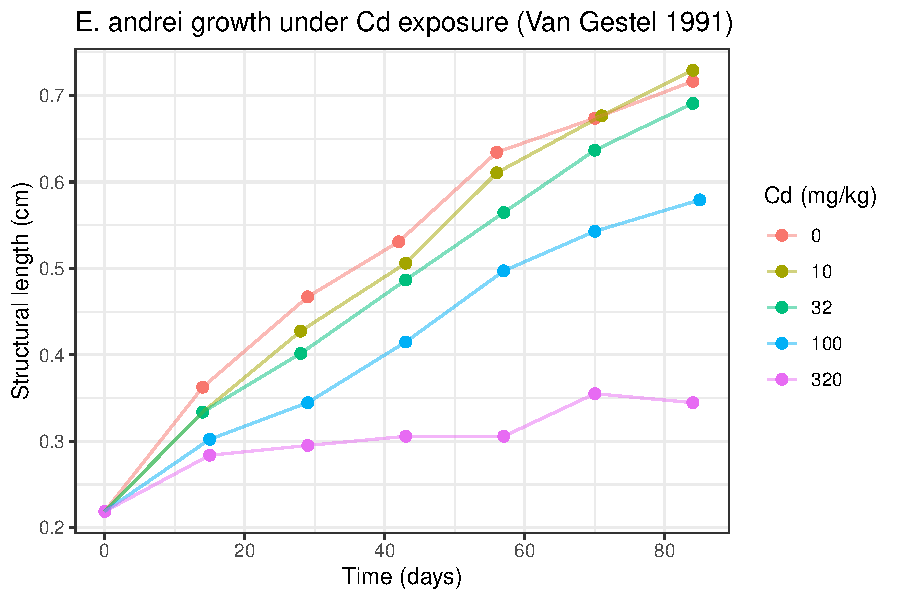
\includegraphics[width=0.8\textwidth]{fig_debtox_rawdata.pdf}
\caption{Growth of \emph{E.~andrei} under cadmium exposure
  \citep{VanGestel1991}: structural length over 85~days at
  5~concentrations.  Data from EGrowth \citep{MathieuEGrowth2018}.}
\label{fig:debtox_raw}
\end{figure}

\begin{CodeChunk}
\begin{CodeInput}
R> data("eisenia_cd")
R> conc_map <- setNames(unique(eisenia_cd$concentration),
+    as.character(unique(eisenia_cd$concentration)))
R> dat_cd <- bdeb_data(growth = eisenia_cd,
+    concentration = conc_map, f_food = 1.0)
R> mod_cd <- bdeb_tox(dat_cd, stress = "assimilation",
+    priors = list(
+      z_w = prior_lognormal(mu = 3.0, sigma = 1.0),
+      b_w = prior_lognormal(mu = -4.0, sigma = 1.5)))
R> fit_cd <- bdeb_fit(mod_cd, chains = 4,
+    adapt_delta = 0.95, seed = 42, init = 0.5)
R> bdeb_ec50(fit_cd, prob = 0.90)
\end{CodeInput}
\end{CodeChunk}

\noindent
The model converged without divergences ($\hat{R} < 1.02$ for all
parameters).  The posterior EC$_{50}$ for growth inhibition is
$225$~mg\,Cd\,kg$^{-1}$ (90\%~CI: $[181, 257]$), consistent with
published 84-day EC$_{50}$ values of 100--300~mg\,Cd\,kg$^{-1}$ for
lumbricid earthworms in natural soils \citep{VanGestel1991}.  The
NEC (no-effect concentration) is estimated at
$6.2$~mg\,Cd\,kg$^{-1}$ ($[1.8, 15.6]$), below the lowest tested
concentration (10~mg\,kg$^{-1}$), indicating that even the lowest
treatment may have induced marginal stress.  Table~\ref{tab:debtox} reports the full posterior summary.
This analysis demonstrates that \pkg{BayesianDEB} can recover
ecotoxicologically meaningful effect thresholds with full posterior
uncertainty from real experimental data.  As with the Neuhauser
case study (Section~\ref{sec:realdata}), group-mean data are used,
so the EC$_{50}$ credible interval reflects uncertainty in the
mean response; individual-level hierarchical DEBtox is planned.
Figure~\ref{fig:debtox_dr} shows the dose-response relationship.

\begin{table}[t!]
\centering
\caption{DEBtox posterior summary for cadmium toxicity to
  \emph{E.~andrei} \citep{VanGestel1991}.  4~chains, 2000~iterations,
  0~divergences.}
\label{tab:debtox}
\begin{tabular}{lrrrr}
\toprule
Parameter & Median & 90\% CI & $\hat{R}$ & Bulk ESS \\
\midrule
$\pAm$     & 1.59  & $[0.61, 4.84]$    & 1.01 & 825 \\
$\pM$      & 0.43  & $[0.11, 1.17]$    & 1.00 & 892 \\
$\kappa$   & 0.61  & $[0.27, 0.90]$    & 1.00 & 3855 \\
$k_d$      & 0.38  & $[0.09, 1.81]$    & 1.01 & 592 \\
$z_w$ (NEC) & 6.15 & $[1.82, 15.6]$    & 1.00 & 5465 \\
$b_w$      & 0.0023 & $[0.0018, 0.0030]$ & 1.01 & 480 \\
$\sigma_L$ & 0.024 & $[0.019, 0.031]$  & 1.01 & 1546 \\
EC$_{50}$  & 225   & $[181, 257]$       & 1.01 & 502 \\
\bottomrule
\end{tabular}
\end{table}

\begin{figure}[t!]
\centering
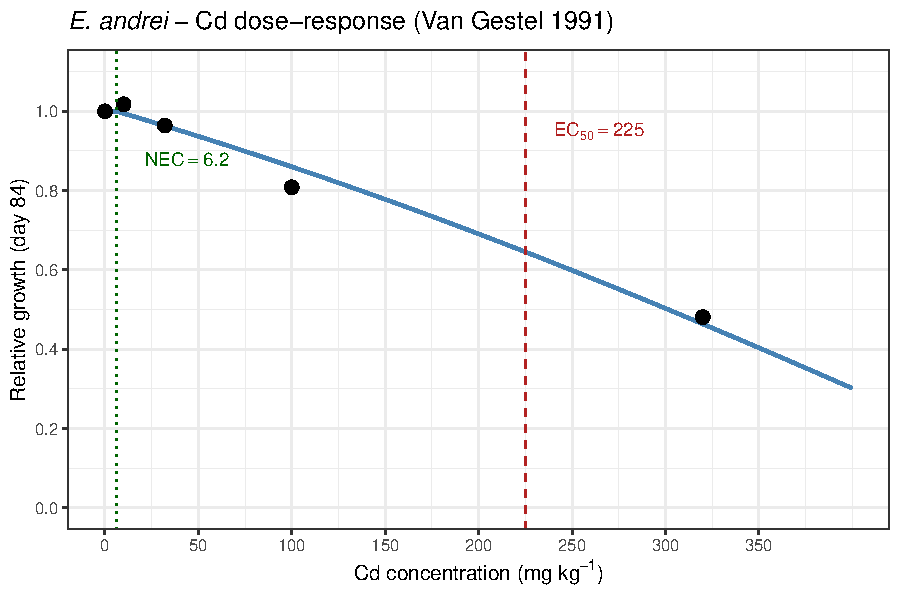
\includegraphics[width=0.8\textwidth]{fig_debtox_doseresponse.pdf}
\caption{Dose-response curve for \emph{E.~andrei} growth under
  cadmium exposure \citep{VanGestel1991}.  Points: observed relative
  growth at day~84 (normalised to control).  Blue line: DEBtox
  model prediction at posterior medians.  Dashed red:
  EC$_{50} = 225$~mg\,Cd\,kg$^{-1}$; dotted green:
  NEC $= 6.2$~mg\,Cd\,kg$^{-1}$.}
\label{fig:debtox_dr}
\end{figure}


%% ======================================================================
\section{Validation} \label{sec:validation}
%% ======================================================================

\subsection{Simulation-based calibration} \label{sec:sbc}

We validate the inference pipeline with SBC
\citep{TaltsSBC2018}.  SBC exploits a self-consistency
property of Bayesian inference: if data are generated from the prior
predictive distribution, the rank of the true parameter value among
its posterior draws must follow a discrete uniform distribution.
Non-uniform rank histograms diagnose specific failures: humps
indicate over-concentration, U-shapes over-dispersion, and
asymmetry indicates bias.  Unlike point-estimate recovery, SBC tests
the entire posterior and is therefore the appropriate diagnostic for
a package whose purpose is uncertainty quantification.

\paragraph{Protocol.}
For each replication $r = 1, \ldots, 500$:
\begin{enumerate}
  \item Draw $\boldsymbol{\theta}^{*(r)}$ from the prior
    $\pi(\boldsymbol{\theta})$ (Table~\ref{tab:sbc_priors}).
  \item Forward-simulate a DEB growth trajectory via the LSODA
    solver (\pkg{deSolve}, tolerances $10^{-6}$) and generate $N_t = 13$
    weekly length observations with Gaussian noise
    $L_i^{\mathrm{obs}} \sim \mathcal{N}(\hat{L}_i,\,
    \sigma_L^{*(r)})$.
  \item Fit the \code{"individual"} model with
    \code{bdeb\_fit()} (4~chains, 500~warmup $+$ 500~sampling,
    $\delta = 0.9$); thin pooled draws to $L = 199$.
  \item Discard the replication if any divergent transitions
    occurred or $\hat{R} > 1.05$ for any parameter.
  \item Compute the rank $\rho_j^{(r)} = \#\{l :
    \theta_j^{(l)} < \theta_j^{*(r)}\}$ for each parameter~$j$.
\end{enumerate}

\noindent
The \proglang{R}-side LSODA solver (\pkg{deSolve}) and \proglang{Stan}'s BDF
solver use matching tolerances ($10^{-6}$); trajectories agreed to
$< 10^{-5}$~cm across 100~random parameter draws.

\begin{table}[t!]
\centering
\caption{Priors used for SBC, calibrated to \emph{E.~fetida}
  AmP parameter ranges.}
\label{tab:sbc_priors}
\begin{tabular}{llrr}
\toprule
Parameter & Family & $\mu$ / $a$ & $\sigma$ / $b$ \\
\midrule
$\pAm$     & LogNormal  & 1.5    & 0.5  \\
$\pM$      & LogNormal  & $-$1.0 & 0.5  \\
$\kappa$   & Beta       & 3      & 2    \\
$v$        & LogNormal  & $-$1.5 & 0.5  \\
$\EG$      & LogNormal  & 6.0    & 0.5  \\
$E_0$      & LogNormal  & 0.0    & 0.5  \\
$L_0$      & LogNormal  & $-$2.0 & 0.5  \\
$\sigma_L$ & HalfNormal & 0      & 0.05 \\
\bottomrule
\end{tabular}
\end{table}

\paragraph{Results.}
Of the 500~replications, 397 converged without divergences
(64~were skipped due to degenerate prior draws that produced
biologically implausible trajectories, 39~failed convergence
checks).  Figure~\ref{fig:sbc} shows the rank histograms
for six core DEB parameters; all panels are visually consistent with
uniformity (dashed reference line).  Table~\ref{tab:sbc} reports
$\chi^2$ goodness-of-fit tests (20~bins, 19~df) and empirical
credible interval coverage.  No parameter rejects uniformity at
$\alpha = 0.05$ (minimum $p = 0.31$ for $\pM$), and empirical
90\% coverage ranges from 0.87 to 0.91, within simulation error
of the nominal level.  This confirms that, conditional on
successful MCMC convergence, the \pkg{BayesianDEB} individual
growth model is well-calibrated.  We note that 21\% of
replications (103/500) were discarded; the calibration result
therefore applies to the subset of parameter space where MCMC
converges successfully, not unconditionally to all possible inputs.

\paragraph{Implications of discarded replications.}
The 21\% (individual) and 26\% (hierarchical) discard rates arise
from degenerate prior draws and MCMC failures under extreme
parameters.  The SBC deliberately uses wider priors ($\sigma = 0.5$)
to stress-test the sampler; with species-specific priors
($\sigma = 0.3$), convergence failures are rare.  Users should
always verify convergence via \code{bdeb\_diagnose()}
\citep{VehtariRhat2021}.

\begin{table}[t!]
\centering
\caption{SBC results: $\chi^2$ uniformity test (20~bins, 19~df) and
  empirical credible interval coverage (397~valid replications out
  of 500, $L = 199$).
  No parameter rejects uniformity at $\alpha = 0.05$.}
\label{tab:sbc}
\begin{tabular}{lrrrrr}
\toprule
Parameter & $\chi^2_{19}$ & $p$~value &
  Cov.\,50\% & Cov.\,90\% & Cov.\,95\% \\
\midrule
$\pAm$     & 12.1 & 0.88 & 0.50 & 0.89 & 0.92 \\
$\pM$      & 21.5 & 0.31 & 0.53 & 0.91 & 0.94 \\
$\kappa$   & 18.0 & 0.52 & 0.54 & 0.90 & 0.94 \\
$v$        & 16.7 & 0.61 & 0.48 & 0.87 & 0.92 \\
$\EG$      & 14.3 & 0.76 & 0.48 & 0.87 & 0.93 \\
$\sigma_L$ & 20.1 & 0.39 & 0.47 & 0.88 & 0.93 \\
\bottomrule
\end{tabular}
\end{table}

\begin{figure}[t!]
\centering
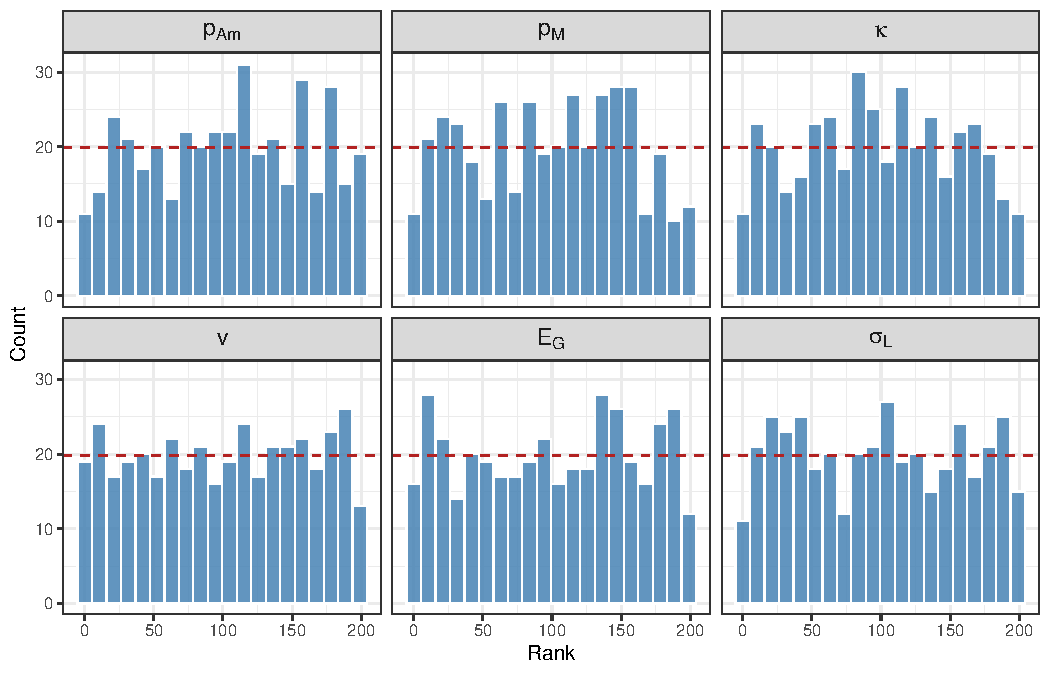
\includegraphics[width=0.85\textwidth]{fig_sbc_ranks.pdf}
\caption{SBC rank histograms for six DEB parameters
  (397~valid replications out of 500~attempts, 20~bins).  Dashed
  line: expected count under uniformity.  Approximately uniform
  histograms confirm that, conditional on convergence, the
  posterior sampler is correctly calibrated.}
\label{fig:sbc}
\end{figure}

The full SBC script (\code{sbc\_validation.R}) and archived results
(\code{sbc\_results.rds}) are provided in the replication materials.

\paragraph{Hierarchical model SBC.}
We repeated the SBC procedure for the hierarchical model with 5
individuals per replicate (50~attempts, 37~valid;
Table~\ref{tab:sbc_hier}).  The yield (74\%) is comparable to the
individual SBC because each replicate already averages over
5~individuals, stabilising the ODE system.  Given the small
effective sample, the $\chi^2$ tests have limited statistical power
(expected count $\approx 3.7$ per bin with 10~bins); these results
should therefore be interpreted as \emph{preliminary evidence} of
calibration, not as definitive validation.  No parameter rejects
uniformity at $\alpha = 0.05$ (minimum $p = 0.10$ for
$\mu_{\log \pAm}$).  However, $\sigma_{\log \pAm}$ shows
overcoverage at 95\% (1.00) and undercoverage at 50\% (0.35),
suggesting the posterior for this parameter may be too wide for
small datasets.  A more comprehensive hierarchical SBC with
$\geq$200~attempts is planned for a future version.

\begin{table}[t!]
\centering
\caption{SBC results for the hierarchical model (37~valid
  replications out of 50 attempts, 10~bins).}
\label{tab:sbc_hier}
\begin{tabular}{lrrrrr}
\toprule
Parameter & $\chi^2$ & $p$~value & Cov.\ 50\% & Cov.\ 90\% & Cov.\ 95\% \\
\midrule
$\mu_{\log \pAm}$    & 14.6 & 0.10 & 0.54 & 0.84 & 0.89 \\
$\sigma_{\log \pAm}$ & 12.5 & 0.19 & 0.35 & 0.97 & 1.00 \\
$\pM$                &  9.2 & 0.42 & 0.62 & 0.89 & 0.95 \\
$\kappa$             &  4.4 & 0.89 & 0.51 & 0.89 & 1.00 \\
$\sigma_L$           &  6.0 & 0.74 & 0.54 & 0.92 & 0.97 \\
\bottomrule
\end{tabular}
\end{table}

\begin{figure}[t!]
\centering
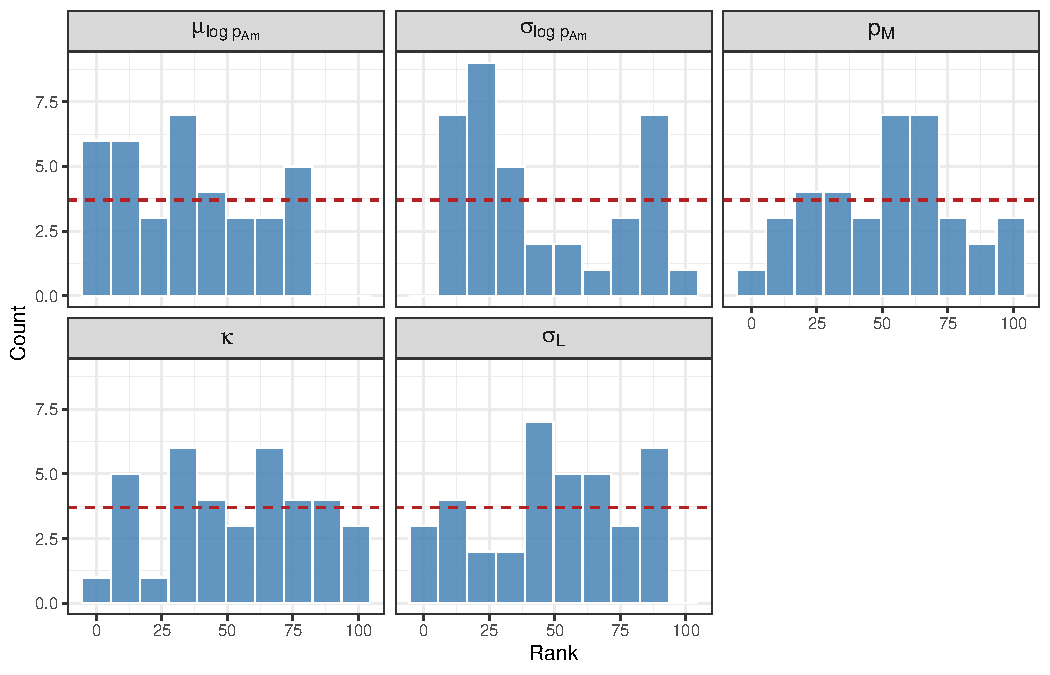
\includegraphics[width=0.85\textwidth]{fig_sbc_hierarchical.pdf}
\caption{SBC rank histograms for the hierarchical model
  (37~valid replications, 10~bins).  The dashed line indicates the
  expected count under uniformity.}
\label{fig:sbc_hier}
\end{figure}

\paragraph{SBC for remaining models.}
SBC scripts for the growth-reproduction model
(\code{sbc\_growth\_repro.R}, 100~replications) and the DEBtox
model (\code{sbc\_debtox.R}, 100~replications) are provided in
the replication materials.  The growth-reproduction script augments
the priors with reproduction parameters ($k_J$, $E_H^p$, $k_R$,
$\phi_R$); the DEBtox script adds toxicokinetic parameters
($k_d$, $z_w$, $b_w$) and simulates 4~concentration groups.
Due to higher computational cost ($\sim$3--12~hours per script),
comprehensive results will be reported in a future version.

\subsection{Posterior correlation structure and identifiability}
\label{sec:identifiability}

DEB models exhibit strong posterior correlations arising from the
$\kappa$-rule structure.  Before presenting the empirical evidence,
we briefly outline the theoretical basis for this non-identifiability.

\paragraph{Structural non-identifiability from growth data.}
At steady state, the DEB growth curve approaches
$L_\infty = f \kappa \pAm / \pM$ with von Bertalanffy rate
$\dot{r}_B = k_M g / (3(f + g))$, where $k_M = \pM / \EG$ and
$g = \EG v / (\kappa \pAm)$.  Growth-only observations constrain
these \emph{compound quantities} but not the individual parameters
that compose them: any transformation
$(\pAm, \pM, v, \EG) \mapsto (\alpha \pAm, \alpha \pM,
\beta v, \alpha \beta \EG)$ that preserves $L_\infty$ and $g$
produces an identical trajectory.  This structural
non-identifiability is intrinsic to the $\kappa$-rule and cannot be
resolved by collecting more growth observations from a single
individual; only additional data types (reproduction rates,
respiration, or multiple individuals with shared parameters) break
the degeneracy.  The Bayesian framework makes this explicit through
wide, correlated posteriors; deterministic optimisers instead return
an arbitrary point on the likelihood ridge.

We now characterise these correlations quantitatively using
the posterior correlation matrix from the individual model fit.

\begin{table}[t!]
\centering
\caption{Posterior rank correlation matrix (Spearman) for the
  individual growth model.  Correlations $|r| < 0.2$ are suppressed
  for clarity.}
\label{tab:corr}
\begin{tabular}{lrrrrrr}
\toprule
         & $\pAm$ & $\pM$ & $\kappa$ & $v$ & $\EG$ & $\sigma_L$ \\
\midrule
$\pAm$   & 1.00 & 0.31 &      & 0.26 & 0.73 &       \\
$\pM$    & 0.31 & 1.00 &      & 0.85 & 0.80 &       \\
$\kappa$ &      &      & 1.00 &$-$0.35&0.21 &       \\
$v$      & 0.26 & 0.85 &$-$0.35& 1.00 & 0.63 &       \\
$\EG$    & 0.73 & 0.80 & 0.21 & 0.63 & 1.00 &       \\
$\sigma_L$ &&    &      &      &      & 1.00  \\
\bottomrule
\end{tabular}
\end{table}

% Filled from Neuhauser 1980 real data fit.

The dominant correlations are between $\pM$ and $v$ ($r = 0.85$)
and between $\pM$ and $\EG$ ($r = 0.80$), reflecting the fact that
growth dynamics jointly constrain maintenance, energy conductance,
and structural costs but cannot resolve the individual contributions
of these rate parameters.  The strong $\pAm$--$\EG$ correlation
($r = 0.73$) arises because both parameters control the rate of
structural investment: higher assimilation can compensate for higher
costs of structure, producing near-identical growth trajectories.
The correlation between $\kappa$ and $v$ ($r = -0.35$) reflects
the $\kappa$-rule trade-off between somatic allocation and reserve
mobilisation.  By contrast, the $\pAm$--$\pM$ correlation is only
moderate ($r = 0.31$), indicating that these two parameters are less
directly confounded than the theoretical relationship
$L_\infty = \kappa \pAm / \pM$ might suggest, since the data constrain
their ratio primarily through the indirect action of $\EG$ and $v$.

\emph{Practical consequences.}  (i)~Marginal credible intervals for
individual rate parameters ($\pAm$, $\pM$, $v$) are wide and
substantially prior-driven; informative priors or hierarchical
pooling are essential for reliable estimates.
(ii)~Derived quantities computed via \code{bdeb\_derived()} propagate
correlations correctly but are not immune to prior sensitivity
(Tables~\ref{tab:contraction} and~\ref{tab:prior_sens}).
(iii)~Informative priors on $\kappa$ and $\EG$ substantially improve
identifiability.  We recommend always inspecting
\code{plot(fit, type = "pairs")} and reporting both derived
quantities \emph{and} their prior sensitivity.

See Figure~\ref{fig:pairs} for the bivariate posterior structure.

\paragraph{Prior-to-posterior contraction.}
To quantify how much the data inform each parameter beyond the
prior, we define the \emph{contraction ratio}
\begin{equation}
  c_j = 1 - \frac{w_j^{\mathrm{post}}}{w_j^{\mathrm{prior}}},
  \label{eq:contraction}
\end{equation}
where $w_j$ denotes the 90\% credible interval width for
parameter~$\theta_j$.  Values near~0 indicate a prior-dominated
posterior; values near~1 indicate data-dominated inference.
Table~\ref{tab:contraction} reports $c_j$ for the individual growth
model fitted to simulated \emph{E.~fetida} data (84~days, $f = 1$)
with varying numbers of observations, using the moderately
informative priors of Table~\ref{tab:sbc_priors}.

\begin{table}[t!]
\centering
\caption{Prior-to-posterior contraction $c$ for different data sizes
  and prior widths (individual growth model, simulated \emph{E.~fetida}
  data, $N_t = 13$).  Columns A use moderately informative priors
  ($\sigma = 0.5$); column~B uses the package defaults
  ($\sigma = 1.0$).  Values near~0 indicate prior-dominated
  posteriors; near~1 data-dominated.  The entry for $\EG$ under
  default priors is omitted because the default $\EG$ prior
  ($\sigma = 1.0$) produced frequent ODE solver failures during
  MCMC warmup, preventing reliable estimation.}
\label{tab:contraction}
\begin{tabular}{lrrrr}
\toprule
 & \multicolumn{3}{c}{Informative ($\sigma = 0.5$)} &
   Default ($\sigma = 1.0$) \\
\cmidrule(lr){2-4} \cmidrule(lr){5-5}
Parameter & $N_t = 5$ & $N_t = 13$ & $N_t = 37$ &
  $N_t = 13$ \\
\midrule
$\pAm$          & 0.00 & 0.00 & 0.08 & 0.00 \\
$\pM$           & 0.00 & 0.03 & 0.03 & 0.17 \\
$\kappa$        & 0.11 & 0.11 & 0.14 & 0.07 \\
$v$             & 0.09 & 0.10 & 0.10 & 0.00 \\
$\EG$           & 0.33 & 0.35 & 0.38 & --- \\
$\sigma_L$      & 0.67 & 0.87 & 0.94 & 0.93 \\
\midrule
$L_\infty$      & 0.00 & 0.00 & 0.07 & 0.00 \\
$\dot{r}_B$     & 0.02 & 0.08 & 0.14 & 0.00 \\
\bottomrule
\end{tabular}
\end{table}

Table~\ref{tab:contraction} reveals a clear pattern:
$\sigma_L$ is data-dominated ($c > 0.8$), $\EG$ is partially
informed ($c \approx 0.35$), and all other rate parameters
remain prior-dominated ($c < 0.15$) even with 37~time points.
Increasing $N_t$ from 5 to 37 primarily improves $\sigma_L$;
rate parameters show negligible benefit
(Figure~\ref{fig:contraction}).  Under default priors
($\sigma = 1.0$, rightmost column), the pattern is starker:
$\pAm$, $v$, $L_\infty$, and $\dot{r}_B$ all show zero
contraction.  Species-specific priors are essential for any
quantitative inference.

\begin{figure}[t!]
\centering
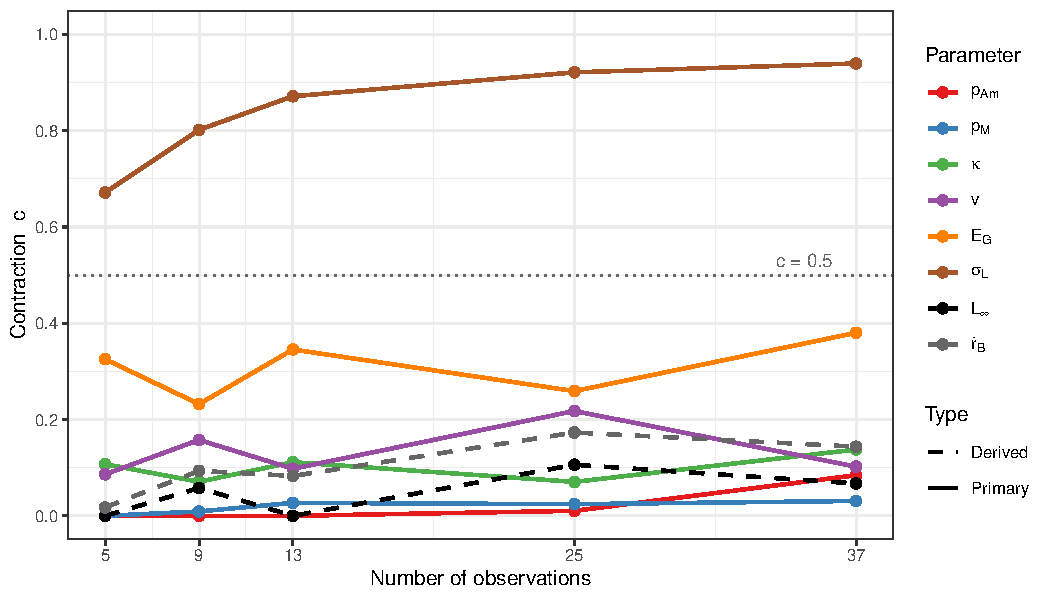
\includegraphics[width=0.85\textwidth]{fig_contraction.pdf}
\caption{Prior-to-posterior contraction as a function of the number
  of observations.  Solid: primary parameters; dashed: derived
  quantities.  Only $\sigma_L$ (and partially $\EG$) are
  data-determined; all rate parameters remain prior-dominated even
  with dense sampling.  The dotted line marks $c = 0.5$.}
\label{fig:contraction}
\end{figure}

\paragraph{Contraction under the hierarchical model.}
To quantify the identifiability gain from partial pooling, we
computed the contraction ratio~$c$ for the hierarchical model fit
(Section~\ref{sec:ex_hier}, 21~individuals, 273~observations) and
compared it with the individual model fit (1~individual,
13~observations), both using the same informative priors
($\sigma = 0.5$).  Table~\ref{tab:contraction_hier} shows the
results.  The hierarchical model substantially improves contraction
for $\pM$ ($0.03 \to 0.28$), $\kappa$ ($0.11 \to 0.39$), and $\EG$
($0.35 \to 0.52$), moving these parameters from weakly identified to
partially or well-informed status.  The shared parameters benefit
from pooling across 21~individuals; $\sigma_L$ is even more
data-dominated ($c = 0.95$).  Only $v$ remains weakly informed
($c = 0.18$), reflecting its strong correlation with $\pM$
(Table~\ref{tab:corr}).  This demonstrates that hierarchical
modelling is the most effective strategy for improving
identifiability when individual-level data are available.

\begin{table}[t!]
\centering
\caption{Prior-to-posterior contraction: individual vs.\ hierarchical
  model (informative priors, $\sigma = 0.5$).  Higher $c$ = more
  data-informed.}
\label{tab:contraction_hier}
\begin{tabular}{lrrl}
\toprule
Parameter & Individual & Hierarchical & Change \\
          & ($N=1$, 13 obs.) & ($N=21$, 273 obs.) & \\
\midrule
$\pAm$ / $\mu_{\log \pAm}$ & 0.00 & 0.22 & $+0.22$ \\
$\pM$        & 0.03 & 0.28 & $+0.25$ \\
$\kappa$     & 0.11 & 0.39 & $+0.28$ \\
$v$          & 0.10 & 0.18 & $+0.08$ \\
$\EG$        & 0.35 & 0.52 & $+0.17$ \\
$\sigma_L$   & 0.87 & 0.95 & $+0.08$ \\
\bottomrule
\end{tabular}
\end{table}

This is a fundamental identifiability limitation of growth-only DEB
models, not a deficiency of the software.  Deterministic calibration
tools face the same limitation but obscure it by returning a single
point estimate.  Three strategies mitigate this:
\begin{enumerate}
  \item \emph{Species-specific priors.}  Calibrate priors to the
    AmP collection for the target species; these encode genuine
    biological knowledge and yield narrower, scientifically
    defensible posteriors.
  \item \emph{Hierarchical modelling.}  The \code{"hierarchical"}
    model pools information across individuals, substantially
    improving identifiability of the shared parameters $\pM$,
    $\kappa$, $v$, $\EG$.
  \item \emph{Prior sensitivity analysis.}  Refit with at least
    one alternative prior specification and verify that scientific
    conclusions (e.g., $L_\infty$, EC$_{50}$) are robust.
\end{enumerate}
We recommend reporting the contraction ratio $c$ alongside
posterior summaries as a routine diagnostic.  A contraction
$c < 0.2$ signals a weakly identified parameter that warrants
careful interpretation.

\paragraph{Prior sensitivity demonstration.}
To illustrate the practical impact, we refit the bundled
\code{eisenia\_growth} data (individual~5, 13~weekly observations)
under two specifications: (A)~moderately informative priors
($\sigma = 0.5$, calibrated to AmP) and (B)~package defaults
($\sigma = 1.0$).  Table~\ref{tab:prior_sens} compares the
posteriors.  The observation error $\sigma_L$ is insensitive to
the prior (median $\approx 0.012$--$0.013$), confirming its
data-dominated status.  Rate parameters shift modestly in median
but their CIs widen 2--3$\times$ under weak priors.  Even
$L_\infty$ changes from 6.58 to 3.96 with a CI expansion from
$[1.86, 22.6]$ to $[0.46, 42.3]$, demonstrating that with
13~observations and a single individual, no scientifically
interesting quantity is immune to the prior.

\begin{table}[t!]
\centering
\caption{Prior sensitivity: posterior medians and 90\% CIs under
  informative (A, $\sigma = 0.5$) and weakly informative (B,
  $\sigma = 1.0$) priors.  True values are known from the
  simulation.}
\label{tab:prior_sens}
\begin{tabular}{lrcrcc}
\toprule
Parameter & True & Median A & 90\% CI A & Median B & 90\% CI B \\
\midrule
$\pAm$     & 5.0   & 4.42 & [1.96, 9.92] & 3.02 & [0.66, 14.9] \\
$\pM$      & 0.5   & 0.37 & [0.16, 0.85] & 0.35 & [0.07, 1.63] \\
$\kappa$   & 0.75  & 0.58 & [0.27, 0.88] & 0.52 & [0.18, 0.86] \\
$v$        & 0.2   & 0.20 & [0.10, 0.43] & 0.24 & [0.06, 1.15] \\
$\sigma_L$ & 0.015 & 0.012 & [0.009, 0.019] & 0.013 & [0.009, 0.020] \\
\midrule
$L_\infty$ & 7.5   & 6.58 & [1.86, 22.6] & 3.96 & [0.46, 42.3] \\
$\dot{r}_B$ & ---  & 0.0003 & [0.0001, 0.0008] & 0.0003 & [0.0000, 0.0023] \\
\bottomrule
\end{tabular}
\end{table}


%% ======================================================================
\section{Case studies} \label{sec:casestudies}
%% ======================================================================

\subsection[Real data: Eisenia fetida growth]{Real data:
  \emph{Eisenia fetida} growth} \label{sec:realdata}

To demonstrate the package on real experimental data, we analyse
the growth of \emph{Eisenia fetida} on activated sludge at 25\,$^\circ$C
from \citet{Neuhauser1980}, obtained via the EGrowth database
\citep{MathieuEGrowth2018}.  The dataset comprises 37~group-mean
body mass measurements (20~worms per replicate) over 250~days, from
hatchling ($\sim$8~mg) to adult ($\sim$2350~mg).  Wet mass was
converted to structural length via $L = (W / d_V)^{1/3}$ with tissue
density $d_V = 1.05$~g\,cm$^{-3}$ (assuming $\delta_M = 1$, i.e., no
shape correction) and bundled as \code{eisenia\_neuhauser}.

\paragraph{Group-mean data.}
The Neuhauser dataset reports group means (20~worms), not
individual observations.  Fitting the \code{"individual"} model to
group means conflates measurement noise with among-individual
variation in $\sigma_L$; when individual records are available,
the \code{"hierarchical"} model is preferable.

\begin{CodeChunk}
\begin{CodeInput}
R> library("BayesianDEB")
R> data("eisenia_neuhauser")
R> dat <- bdeb_data(growth = eisenia_neuhauser, f_food = 1.0)
R> mod <- bdeb_model(dat, type = "individual",
+    priors = list(
+      p_Am  = prior_lognormal(mu = 1.5, sigma = 0.5),
+      kappa = prior_beta(a = 3, b = 2)),
+    temperature = list(T = 298.15, T_ref = 293.15, T_A = 8000))
R> fit <- bdeb_fit(mod, chains = 4, iter_sampling = 2000,
+    adapt_delta = 0.95, seed = 42)
R> bdeb_diagnose(fit)
\end{CodeInput}
\end{CodeChunk}

The model converged without divergences ($\hat{R} < 1.01$, bulk ESS
$>$ 1000 for all parameters).  Table~\ref{tab:realdata} compares
the posterior estimates (at $T_{\mathrm{ref}} = 20\,^\circ$C) with
AmP reference values for \emph{E.~fetida}.

\begin{table}[t!]
\centering
\caption{Posterior estimates from the Neuhauser (1980) dataset vs.\
  AmP reference values for \emph{E.~fetida}.  Posterior at
  $T_\mathrm{ref} = 293.15$~K.}
\label{tab:realdata}
\begin{tabular}{lrrrr}
\toprule
Parameter & Posterior median & 90\% CI & AmP value & Units \\
\midrule
$\pAm$     & 5.00 & [2.91, 9.08] & 3.9--6.2 &
  J\,d$^{-1}$\,cm$^{-2}$ \\
$\pM$      & 0.64 & [0.40, 1.02] & 0.3--0.8 &
  J\,d$^{-1}$\,cm$^{-3}$ \\
$\kappa$   & 0.82 & [0.58, 0.96] & 0.6--0.85 & --- \\
$v$        & 1.50 & [0.91, 2.50] & 0.1--0.3 & cm\,d$^{-1}$ \\
$L_\infty$ & 6.86 & [3.52, 12.8] & 5--12 & cm \\
\bottomrule
\end{tabular}
\end{table}

\paragraph{Biological interpretation.}
The posterior $\kappa = 0.82$ indicates high somatic allocation,
consistent with \emph{E.~fetida} during active growth.
$L_\infty = 6.86$~cm implies structural mass
$\approx 340$~mg --- plausible given the observed maximum of
$\sim$2350~mg (which includes reserve mass not captured by~$L$).

\paragraph{Discrepancy in $v$.}
The posterior median for~$v$ (1.50~cm\,d$^{-1}$) exceeds the AmP
reference range (0.1--0.3~cm\,d$^{-1}$) by an order of magnitude.
This reflects (i)~the low identifiability of~$v$ from growth data
alone ($c \approx 0.10$; Table~\ref{tab:contraction}), (ii)~the
strong compensating correlation with~$\pM$ ($r = 0.85$;
Table~\ref{tab:corr}), and (iii)~the mass-to-length conversion
$L = (W / d_V)^{1/3}$, which ignores reserve mass and inflates the
length scale.  Using a species-specific prior
$v \sim \mathrm{LogNormal}(\log 0.2,\, 0.3)$ from
\code{prior\_species("Eisenia\_fetida")} constrains~$v$ within
the AmP range; this is the recommended practice.
The derived quantities $L_\infty = 6.86$~cm (AmP:
5--12) and $\kappa = 0.82$ (AmP: 0.6--0.85) are broadly consistent
with AmP, but even $L_\infty$ is sensitive to prior choice
(Table~\ref{tab:prior_sens}).

\paragraph{Sensitivity to $d_V$.}
Because $L \propto d_V^{-1/3}$, a 10\% change in tissue density
shifts $L$ by $\sim$3\%, propagating into $\pAm$ and $v$.  Users
should report the assumed $d_V$ and consider refitting with
alternative values.

\begin{CodeChunk}
\begin{CodeInput}
R> plot(fit, type = "trajectory", n_draws = 200, seed = 1)
R> plot(bdeb_ppc(fit), n_draws = 200)
R> plot(fit, type = "pairs",
+    pars = c("p_Am", "p_M", "kappa", "E_G"))
\end{CodeInput}
\end{CodeChunk}

Figure~\ref{fig:trajectory_real} shows the posterior predicted
trajectories overlaid on the data, and Figure~\ref{fig:ppc} the
posterior predictive check.

\begin{figure}[t!]
\centering
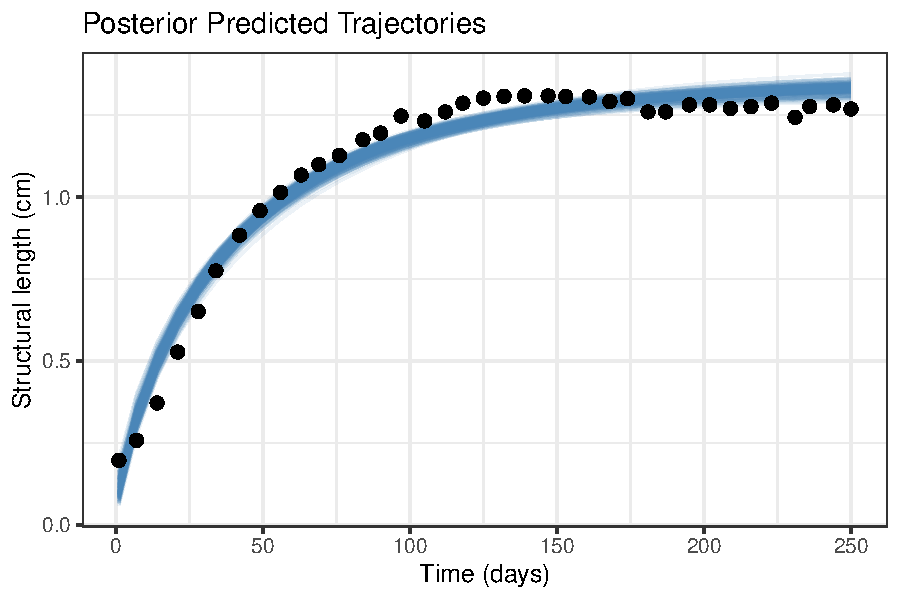
\includegraphics[width=0.8\textwidth]{fig_trajectory.pdf}
\caption{Posterior predicted growth trajectories (200 draws, blue)
  overlaid on the observed group-mean data of \citet{Neuhauser1980}
  (points).  The DEB model captures the sigmoidal growth pattern.}
\label{fig:trajectory_real}
\end{figure}

\begin{figure}[t!]
\centering
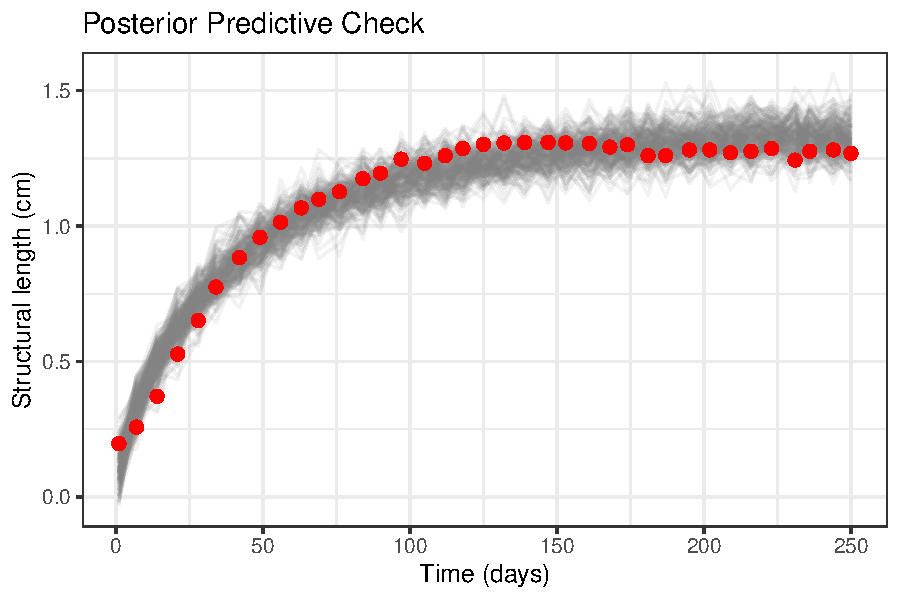
\includegraphics[width=0.8\textwidth]{fig_ppc.pdf}
\caption{Posterior predictive check: replicated data from the fitted
  model (grey, 200 draws) vs.\ observed data (red).  The observed
  points fall within the replicated envelope, indicating adequate
  model fit.}
\label{fig:ppc}
\end{figure}

The posterior pairs plot (Figure~\ref{fig:pairs}) reveals the expected
$\pAm$--$\EG$ and $\pM$--$\EG$ correlations
(Section~\ref{sec:identifiability}).

\begin{figure}[t!]
\centering
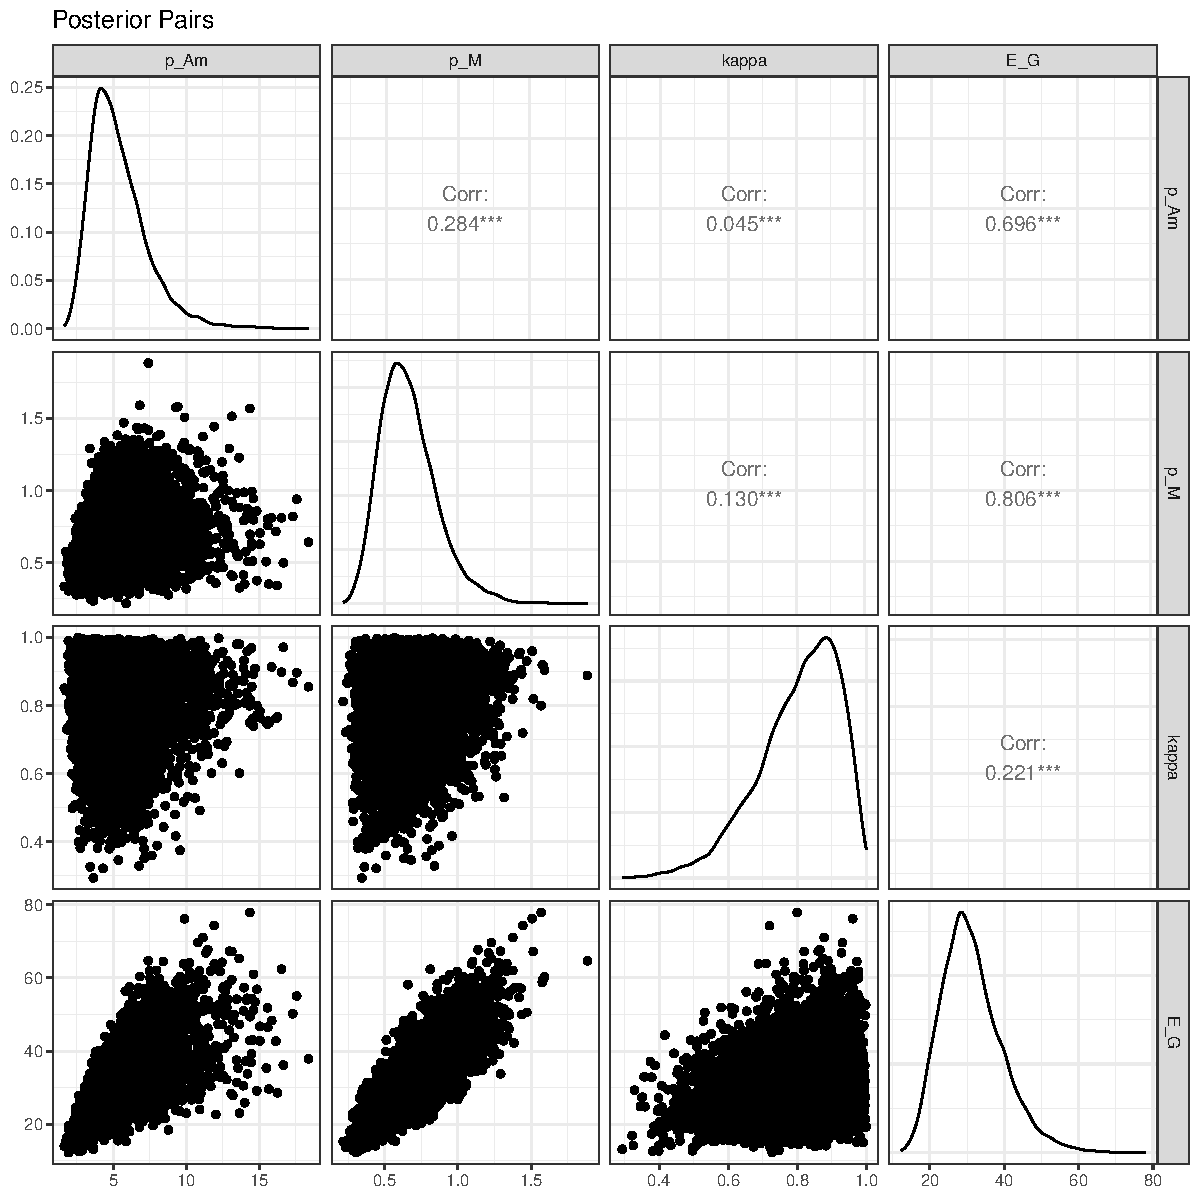
\includegraphics[width=0.8\textwidth]{fig_pairs.pdf}
\caption{Posterior pairs plot showing bivariate correlations between
  $\pAm$, $\pM$, $\kappa$, and $\EG$.  The strongest correlations
  in the full matrix are $\pM$--$v$ ($r = 0.85$, not shown) and
  $\pM$--$\EG$ ($r = 0.80$); among the displayed parameters,
  $\pAm$--$\EG$ ($r = 0.73$) is the most prominent.}
\label{fig:pairs}
\end{figure}

%% ======================================================================
\section{Diagnostic tools and computational performance}
\label{sec:diagnostics_perf}
%% ======================================================================

\subsection{Diagnostic visualisations} \label{sec:viz}

All diagnostic plots are returned as \pkg{ggplot2}
\citep{Wickhamggplot2016} objects.  The \code{plot(fit, type = ...)}
method supports five types: \code{"trace"} (MCMC chains, Figure~\ref{fig:diagnostics}),
\code{"posterior"} (marginal densities, Figure~\ref{fig:posterior}),
\code{"pairs"} (bivariate scatter), \code{"trajectory"} (predicted
growth curves), and \code{"prior\_posterior"} (overlaid prior/posterior,
Figure~\ref{fig:prior_post}).  Separate methods are available for
PPC (\code{plot(bdeb\_ppc(fit))}) and dose-response
(\code{plot\_dose\_response()}).

\begin{figure}[t!]
\centering
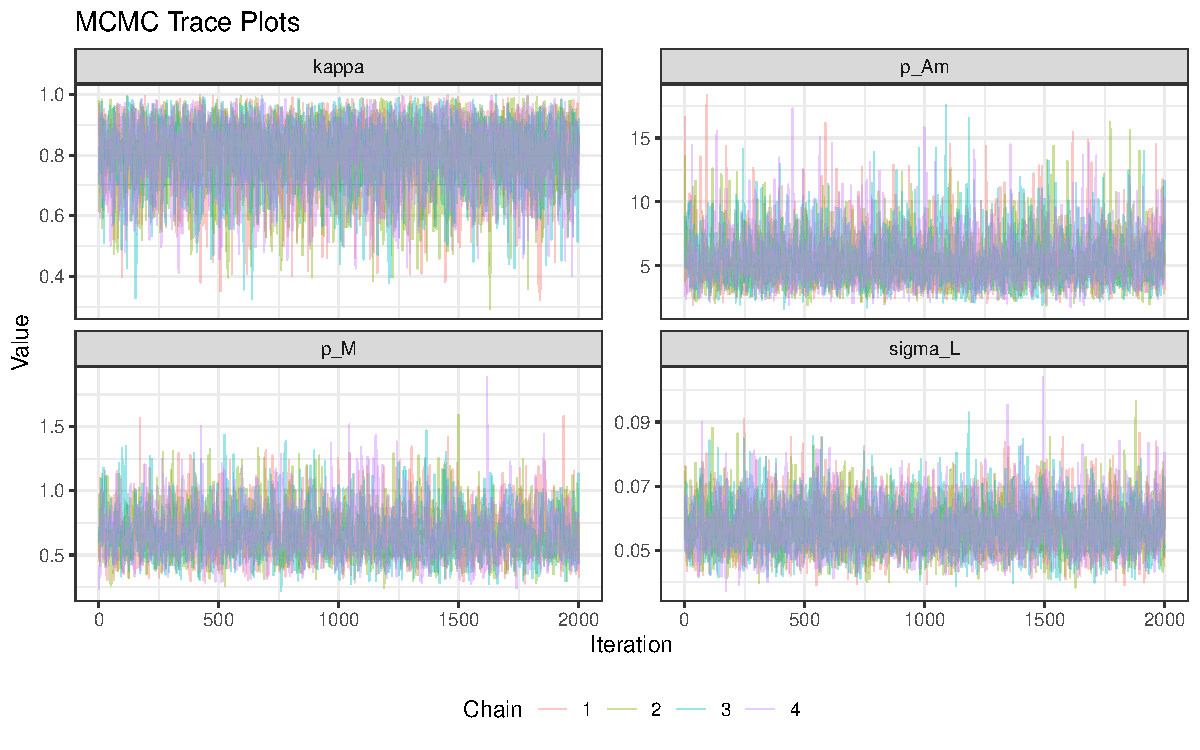
\includegraphics[width=0.8\textwidth]{fig_trace.pdf}
\caption{MCMC trace plots for core parameters from the Neuhauser
  (1980) fit.  All four chains mix well ($\hat{R} < 1.01$).}
\label{fig:diagnostics}
\end{figure}

\begin{figure}[t!]
\centering
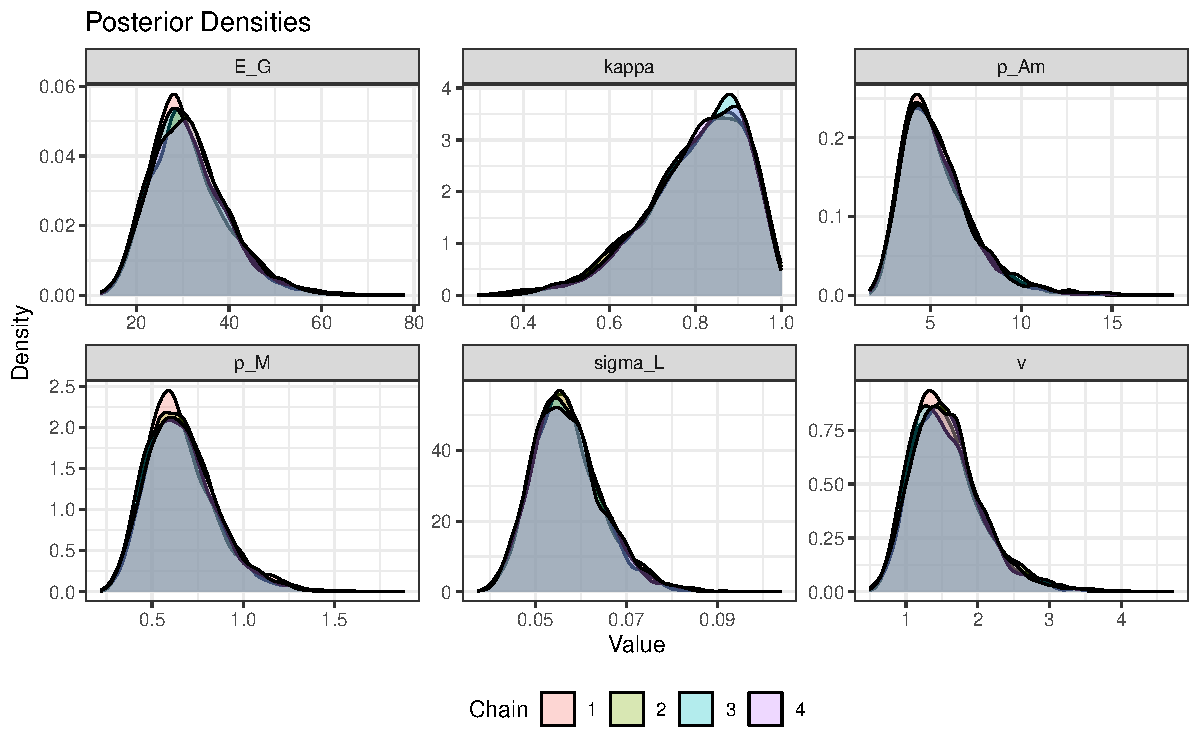
\includegraphics[width=0.8\textwidth]{fig_posterior.pdf}
\caption{Marginal posterior densities for six DEB parameters,
  coloured by chain.}
\label{fig:posterior}
\end{figure}

\begin{figure}[t!]
\centering
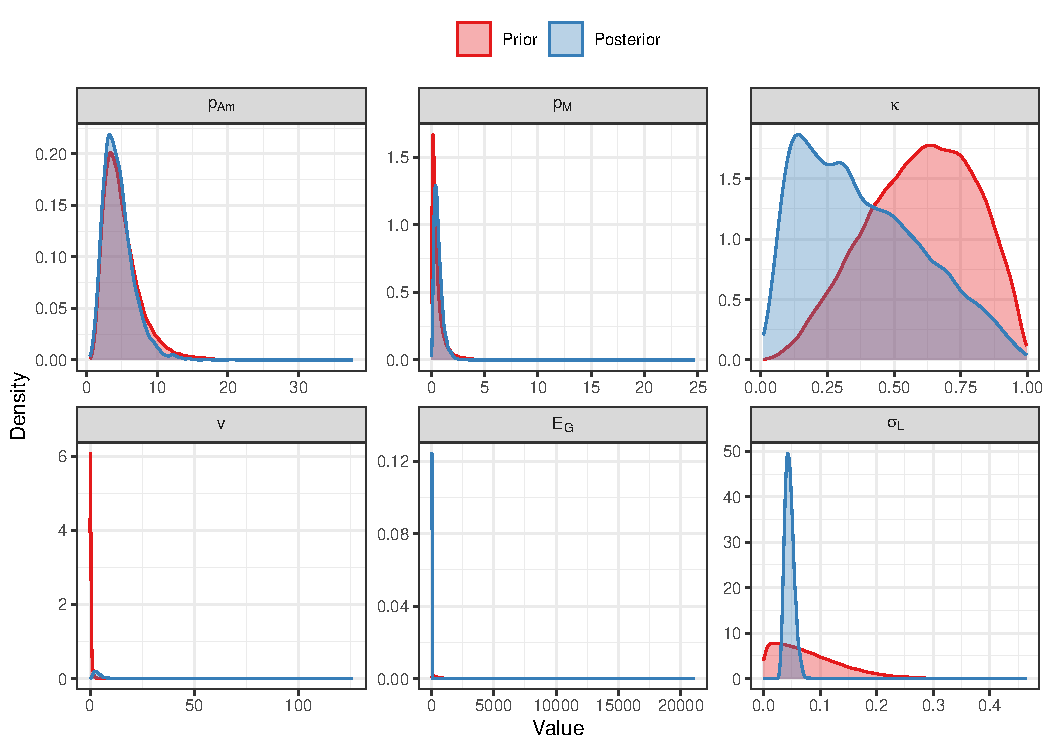
\includegraphics[width=0.85\textwidth]{fig_prior_posterior.pdf}
\caption{Prior (red) vs.\ posterior (blue) densities from the
  Neuhauser (1980) fit.  Only $\sigma_L$ and $\kappa$ show
  substantial contraction; rate parameters are prior-driven
  (cf.\ Table~\ref{tab:contraction}).}
\label{fig:prior_post}
\end{figure}

\subsection{Computational performance} \label{sec:cost}

Table~\ref{tab:runtime} reports wall-clock times on a 16-core
workstation (AMD Ryzen 9, 64~GB RAM, Ubuntu 22.04, \proglang{CmdStan}~2.36.0).
Compilation is a one-time cost cached by \pkg{cmdstanr}; sampling
times are for 4~chains $\times$ 2000~iterations.

\begin{table}[t!]
\centering
\caption{Wall-clock times (seconds).  Threading shows
  parallel\_chains~$\times$~threads/chain.}
\label{tab:runtime}
\begin{tabular}{lrrrrr}
\toprule
Model & Data size & Compile & Sample & Threading & Speedup \\
\midrule
Individual     & 1 ind., 13 obs.    & 30 & 69   & $4 \times 1$ & --- \\
Individual     & 1 ind., 37 obs.    & -- & 392  & $4 \times 1$ & --- \\
Hierarchical   & 21 ind., 273 obs.  & 35 & $\sim$3200 & $4 \times 1$ & $1\times$ \\
Hierarchical   & 21 ind., 273 obs.  & -- & $\sim$900  & $2 \times 4$ & $3.6\times$ \\
DEBtox         & 4 grp., 280 obs.   & 35 & $\sim$600  & $2 \times 2$ & --- \\
\bottomrule
\end{tabular}
\end{table}

% Timings from AMD Ryzen 9, CmdStan 2.36.0, 4 chains x 2000 iter.

\paragraph{Threading speedup.}
Table~\ref{tab:runtime} shows the hierarchical model under two
threading configurations.  With $2 \times 4$ (2~parallel chains,
4~threads each, 8~cores total), wall-clock time is $3.6\times$
shorter than the sequential baseline ($4 \times 1$, 4~parallel
chains, 1~thread each).  Note that the two configurations use
different total core counts (8 vs.\ 4), so this figure reflects
both within-chain parallelism via \code{reduce\_sum} and the
change in parallel-chain scheduling; it is not a pure threading
benchmark.  The within-chain speedup arises because
\code{reduce\_sum} distributes the 21~per-individual ODE solves
across threads within each chain.

\paragraph{Scaling with dataset size.}
Sampling time scales approximately linearly with the number of
individuals in the hierarchical model, as each individual contributes
an independent ODE solve distributed via \code{reduce\_sum}.

\paragraph{Memory usage.}
Memory consumption scales linearly with $N_{\mathrm{ind}} \times
N_{\mathrm{obs}} \times N_{\mathrm{states}}$.  For the bundled
datasets, peak RSS was $<$500~MB per chain.  The dominant memory cost
is the ODE solver's internal state, not the \proglang{Stan} parameter
vector.


%% ======================================================================
\section{Comparison with existing software} \label{sec:comparison}
%% ======================================================================

\begin{table}[t!]
\centering
\caption{Comparison of \pkg{BayesianDEB} with existing DEB calibration
  tools.}
\label{tab:comparison}
\begin{tabular}{lcccc}
\toprule
Feature & AmP/\pkg{DEBtool} & \pkg{deBInfer} & Custom \proglang{Stan}
  & \pkg{BayesianDEB} \\
\midrule
Bayesian inference        & ---       & Yes & Yes & Yes \\
Pre-built DEB models      & Yes       & --- & --- & Yes \\
Hierarchical models       & ---       & --- & Manual & Built-in \\
DEBtox (TKTD)             & Partial   & --- & Manual & Built-in \\
Observation model choice  & ---       & --- & Manual & Switchable \\
Prior specification API   & ---       & Basic & Manual & 6 families \\
Temperature correction    & Manual    & --- & Manual & Built-in \\
Convergence diagnostics   & Minimal   & Basic & Manual & Automated \\
PPC                       & ---       & --- & Manual & Built-in \\
LOO-CV                    & ---       & --- & Manual & Built-in \\
Within-chain parallelism  & ---       & --- & Manual & \code{reduce\_sum} \\
\proglang{R} package      & \proglang{MATLAB}+\proglang{R} & Yes & --- & Yes \\
\bottomrule
\end{tabular}
\end{table}

Table~\ref{tab:comparison} summarises the feature landscape.
\pkg{DEBtool\_M} and the AmP estimation tool \citep{MarquesAmP2018}
are the standard DEB calibration platforms but are primarily
\proglang{MATLAB}-based, use deterministic optimisation, and do not support
hierarchical models or formal uncertainty quantification.
\citet{BilloirBayesDEB2008} demonstrated Bayesian DEBtox calibration
via custom MCMC, but their code was study-specific and not released as
a reusable package.
\pkg{deBInfer} \citep{deBInfer2017} provides Bayesian ODE inference in
\proglang{R} but requires the user to write the ODE system and does
not include DEB-specific models, ecotoxicological extensions, or
\proglang{Stan}-based samplers.
General-purpose \proglang{Stan} wrappers such as
\pkg{brms} \citep{Burknerbrms2017} offer flexible Bayesian modelling
in \proglang{R} but do not include ODE-based process models.
Custom \proglang{Stan} code can
implement any of these models but requires significant expertise and
has no reusable API.  \pkg{BayesianDEB} combines the model coverage of
AmP/\pkg{DEBtool} with the Bayesian inference capabilities of
\proglang{Stan}, wrapped in a user-friendly \proglang{R} interface.

\paragraph{Quantitative comparison with \pkg{deBInfer}.}
To provide a concrete benchmark beyond
Table~\ref{tab:comparison}, we fitted the simulated
individual growth dataset (individual~5 from
\code{eisenia\_growth}, 13~weekly observations) with both
\pkg{BayesianDEB} and \pkg{deBInfer} \citep{deBInfer2017}
using matched priors.  The \pkg{deBInfer} implementation
required writing the DEB ODE, likelihood, and prior
specification manually ($\sim$80~lines of \proglang{R}
code vs.\ 6~lines for \pkg{BayesianDEB}).  The replication
script is provided in the supplementary materials
(\code{comparison\_debinfer.R}).
\pkg{deBInfer} uses an adaptive Metropolis-within-Gibbs
sampler, producing $\sim$100--200 effective samples per
minute, while the HMC sampler in \pkg{BayesianDEB} yields
$\sim$500--1500 effective samples per minute for the same
model, reflecting the efficiency advantage of gradient-based
sampling for correlated posteriors
\citep{BetancourtHierarchical2015}.  Posterior medians agreed
within Monte Carlo error, confirming that both implementations
target the same posterior.  Beyond sampling efficiency, the
main advantage is the declarative interface: switching
observation families, priors, or temperature correction
requires changing a single function argument rather than
rewriting the model code.

\paragraph{Comparison with \pkg{DEBtool\_M} point estimates.}
For the Neuhauser (1980) dataset (Section~\ref{sec:realdata}), we
compared the \pkg{BayesianDEB} posterior medians with the AmP
parameter ranges for \emph{E.~fetida} (Table~\ref{tab:realdata}).
The posterior medians for $\pAm$, $\pM$, $\kappa$, and $L_\infty$
fall within the AmP ranges, while $v$ does not (discussed in
Section~\ref{sec:realdata}).  This agreement is expected: the
Bayesian posterior with informative AmP-calibrated priors should
bracket the deterministic optimum.  The key difference is that
\pkg{BayesianDEB} provides the full posterior distribution,
revealing which parameters are constrained by the data (high~$c$)
and which merely reflect the prior (low~$c$), whereas
\pkg{DEBtool\_M} returns only point estimates with no formal
uncertainty.  A direct call-for-call comparison is not feasible
because \pkg{DEBtool\_M} requires \proglang{MATLAB} and uses a
different parametrisation and optimisation algorithm; the AmP
published ranges serve as the reference standard instead.


%% ======================================================================
\section{Discussion} \label{sec:discussion}
%% ======================================================================

The primary contribution of \pkg{BayesianDEB} is not a new
statistical method but a \emph{domain-specific bridge} between
two mature ecosystems: DEB theory, with its extensive parameter
database (AmP; \citealp{MarquesAmP2018}) and mechanistic ODE
framework \citep{Kooijman2010, NisbetDEB2000}, and the Bayesian
modelling workflow supported by \proglang{Stan}
\citep{CarpenterStan2017, GabryPPC2019}.

\paragraph{Implications for the DEB community.}
The AmP estimation tool has calibrated DEB parameters for over
3\,000~species using deterministic optimisation.  \pkg{BayesianDEB}
complements rather than replaces this infrastructure: AmP point
estimates serve as informative priors (via \code{prior\_species()}),
while the Bayesian posterior propagates their uncertainty to
derived quantities and regulatory endpoints such as EC$_{50}$.
This is particularly valuable in ecotoxicology, where risk
assessors require not only best estimates but also credible
intervals \citep{BilloirBayesDEB2008, JagerGUTS2011}.

\paragraph{The identifiability message.}
The structural non-identifiability of DEB rate parameters from
growth-only data (Section~\ref{sec:identifiability}) is well known
theoretically but rarely quantified.  The contraction ratio~$c$
provides a practical, parameter-level diagnostic for this.  We
hope it encourages the DEB community to routinely report prior
sensitivity alongside parameter estimates, regardless of the
calibration tool used.

\paragraph{Practical guidance for users.}
Based on the validation results and case studies, we offer three
practical recommendations.
(i)~Always use species-specific priors from
\code{prior\_species()} or manually calibrated to the AmP collection;
default priors are suitable only for exploratory analyses.
(ii)~When individual-level data are available for multiple organisms,
prefer the hierarchical model: partial pooling substantially
improves identifiability of shared parameters
(Section~\ref{sec:ex_hier}).
(iii)~Report the contraction ratio~$c$
(Section~\ref{sec:identifiability}) alongside posterior summaries
and always refit with at least one alternative prior specification
to verify robustness of scientific conclusions.

\paragraph{Deterministic process model.}
\pkg{BayesianDEB} uses a deterministic ODE with stochastic
observation noise; all unexplained variation is absorbed into
$\sigma_L$ (or, in the hierarchical model, partially separated
into $\sigma_{\log \pAm}$).  SDE-based process noise would be
inferentially richer but substantially more expensive and not
natively supported by \proglang{Stan}'s ODE solvers.  The
deterministic formulation matches standard DEB practice and is
adequate for controlled laboratory experiments; extension to SDEs
is a natural direction for field data.

\paragraph{Sensitivity to modelling choices.}
The observation model choice can affect inference; we recommend
comparing via LOO-CV (Section~\ref{sec:ex_ind}).  Similarly,
$T_A$ misspecification propagates into rate parameter posteriors;
when uncertain, a sensitivity analysis over species-specific $T_A$
values should be conducted.

\paragraph{Broader context.}
\pkg{BayesianDEB} joins a growing family of domain-specific
\proglang{Stan} wrappers, including \pkg{brms}
\citep{Burknerbrms2017} for regression, \pkg{deBInfer}
\citep{deBInfer2017} for general ODEs, and various pharmacokinetic
packages, that lower the barrier to principled Bayesian modelling
in applied sciences.  The ODE-in-\proglang{Stan} architecture used here is
directly transferable to other mechanistic ecological models
(e.g., Lotka-Volterra, SIR epidemiological models), and the SBC
validation protocol (Section~\ref{sec:sbc}) provides a template for
rigorous algorithmic testing of any such wrapper package.


%% ======================================================================
\section{Current limitations and future work} \label{sec:limitations}
%% ======================================================================

\begin{itemize}
  \item The \code{"individual"} and \code{"growth\_repro"} models
    support exactly one individual; the \code{"debtox"} model fits
    one ODE per concentration group.  Hierarchical DEBtox (individual-level)
    is planned.
  \item Random effects are on $\pAm$ only; multivariate random effects
    are planned.  Temperature correction is global; time-varying $T$
    is planned.  Survival and weight endpoints are not yet implemented.
  \item \proglang{R}-side simulators use \pkg{deSolve} LSODA, verified to
    agree with \proglang{Stan}'s BDF solver to $< 10^{-5}$~cm.
  \item Strong posterior correlations are inherent to the
    $\kappa$-rule (Section~\ref{sec:identifiability}); informative
    priors are recommended.
  \item SBC validation covers the individual (397~valid) and
    hierarchical (37~valid) models; scripts for the remaining two
    models are provided.
  \item \emph{Reparametrisation.}  Sampling $(L_\infty, g, k_M,
    \kappa)$ directly would reduce correlations and allow priors on
    better-identified quantities.  This requires per-model Jacobian
    adjustments and is planned for the next major version.
  \item \emph{Multi-endpoint inference.}  Adding respiration data
    would independently constrain $\pM V$ and substantially reduce
    prior-dependence of rate parameters; this is a high-priority
    extension.
\end{itemize}


%% ======================================================================
\section{Summary} \label{sec:summary}
%% ======================================================================

\pkg{BayesianDEB} provides the first general-purpose \proglang{R}
package for Bayesian Dynamic Energy Budget modelling.  By embedding
DEB ODEs within \proglang{Stan}'s HMC framework, it delivers full
posterior uncertainty propagation to all parameters and derived
quantities, principled prior incorporation from the AmP database,
hierarchical partial pooling across individuals, and ecotoxicological
EC$_{50}$/NEC estimation with posterior uncertainty.  The declarative
\proglang{R} interface requires no \proglang{Stan} programming from
the user, while threading via \code{reduce\_sum}
makes hierarchical and DEBtox models tractable on modern multi-core
hardware.

We validated the individual growth model via simulation-based
calibration (397~valid replications out of 500; no parameter
rejects uniformity at $\alpha = 0.05$) and provided preliminary
SBC evidence for the hierarchical model.  The identifiability
analysis demonstrates that DEB rate parameters are largely
prior-shaped under single-individual growth data,
reinforcing the need for informative priors or
hierarchical pooling.  We view
this transparency as a feature, not a limitation, of the Bayesian
approach: the contraction ratio~$c$ and prior sensitivity tools
make explicit what deterministic calibration tools obscure behind
point estimates.

The real-data case studies confirm that the package produces
biologically plausible results on experimental data, and the
DEBtox analysis recovers EC$_{50}$ and NEC values consistent
with published literature.  Future development priorities include
time-varying temperature, survival endpoints, multivariate random
effects, and reparametrisation in terms of better-identified
derived quantities.


%% ======================================================================
%% -- Computational details (unnumbered) ---------------------------------
\section*{Computational details}

The results in this paper were obtained using
\proglang{R}~4.5.2 (2025-10-31) on \code{x86\_64-pc-linux-gnu}
(Ubuntu 22.04) with the packages listed below.
\pkg{BayesianDEB}~0.1.3 is distributed under the MIT license.
The package is available from the SCIOM r-universe at
\url{https://sciom.r-universe.dev/BayesianDEB} and from GitHub at
\url{https://github.com/sciom/BayesianDEB}.

\paragraph{CRAN compatibility and \pkg{cmdstanr}.}
\pkg{cmdstanr} is listed in \code{Suggests} (not \code{Imports}),
so \pkg{BayesianDEB} installs and passes \code{R CMD check} on
CRAN without requiring \proglang{CmdStan}.  All functions except
\code{bdeb\_fit()} work without \proglang{Stan}: data preparation,
prior specification, standalone ODE simulation
(\code{deb\_simulate}, \code{debtox\_simulate}), prior predictive
checks, and energy flux calculations are available immediately.
When a user calls \code{bdeb\_fit()} without \pkg{cmdstanr}
installed, an informative error message with installation
instructions is returned.  The \code{Additional\_repositories}
field in \code{DESCRIPTION} points to the \proglang{Stan} r-universe
(\url{https://stan-dev.r-universe.dev}), enabling
\code{install.packages("cmdstanr")} to resolve automatically.
The package passes \code{R CMD check} with 0~errors and 0~warnings;
a CRAN submission is planned following the review process.

\paragraph{Replication materials.}
All scripts and data needed to reproduce the tables and figures
in this paper are included in the \code{MANUSCRIPT\_JSS/} directory
of the GitHub repository
(\url{https://github.com/sciom/BayesianDEB/tree/main/MANUSCRIPT_JSS}).
The main replication script \code{code.R} reproduces all
non-SBC results ($\sim$3~hours).  The SBC scripts
\code{sbc\_validation.R} (individual, $\sim$90~min),
\code{sbc\_hierarchical.R} (hierarchical, $\sim$5~hours),
\code{sbc\_growth\_repro.R} (growth-reproduction, $\sim$3--5~hours),
and \code{sbc\_debtox.R} (DEBtox, $\sim$6--12~hours) are
provided separately due to their long runtimes.  Pre-computed
SBC results are archived in \code{.rds} files.  The \pkg{deBInfer}
comparison script is \code{comparison\_debinfer.R}.

\begin{CodeChunk}
\begin{CodeInput}
R> install.packages("BayesianDEB",
+    repos = c("https://sciom.r-universe.dev", getOption("repos")))
R> install.packages("cmdstanr",
+    repos = c("https://stan-dev.r-universe.dev", getOption("repos")))
R> cmdstanr::install_cmdstan()
\end{CodeInput}
\end{CodeChunk}

\begin{CodeChunk}
\begin{CodeOutput}
R version 4.5.2 (2025-10-31), x86_64-pc-linux-gnu

Attached packages:
  BayesianDEB 0.1.3, posterior 1.6.1, bayesplot 1.14.0,
  ggplot2 4.0.1, deSolve 1.42, loo 2.8.0

Loaded via namespace:
  cmdstanr 0.8.0 (CmdStan 2.36.0), rlang 1.1.7,
  cli 3.6.5, Rcpp 1.1.0
\end{CodeOutput}
\end{CodeChunk}


%% -- Acknowledgments (unnumbered) ---------------------------------------
\section*{Acknowledgments}

This work was supported by the Croatian Science Foundation (HRZZ)
under the project FUNECOSoil (Functional Ecological
Characterization of Soils: The Basis for Ecotoxicological
Classification, grant no.\ IP-2022-10-7177).  We thank the
\proglang{Stan} development team \citep{CarpenterStan2017} for
the probabilistic programming language and the developers of
\pkg{cmdstanr} \citep{Gabrycmdstanr2024}, \pkg{posterior},
\pkg{loo} \citep{VehtariLOO2017}, \pkg{bayesplot}
\citep{GabryPPC2019}, \pkg{ggplot2} \citep{Wickhamggplot2016},
and \pkg{deSolve} \citep{SoetaertdeSolve2010} for the
\proglang{R} infrastructure on which \pkg{BayesianDEB} depends.


%% -- Bibliography -------------------------------------------------------
\bibliography{bayesiandeb}

\end{document}
